\documentclass[journal]{IEEEtran}
\usepackage{cite}
\usepackage{amsmath,amssymb,amsfonts,amsthm}
\newtheorem*{problem}{Problem Statement}
\usepackage{graphicx}
\usepackage{booktabs}
\usepackage{multirow}
\usepackage{array}
\usepackage{algorithm}
\usepackage{algorithmic}
\usepackage{url}
\usepackage[hidelinks]{hyperref}
\usepackage{xcolor}
\usepackage{caption}
\usepackage{adjustbox}
\usepackage{dblfloatfix}
\usepackage{cuted}
\usepackage{float}
%% ── Theorem environments ─────────────────────────────────────────────────

\setlength{\textfloatsep}{16pt}
\setlength{\floatsep}{6pt}
\setlength{\intextsep}{6pt}
\setlength{\belowcaptionskip}{0pt}
\setlength{\abovecaptionskip}{0pt}
%% =========================================================================
\begin{document}
	%% =========================================================================
	\title{JUCO: A Joint Uncertainty-Calibrated Optimisation Framework for ICU Mortality Prediction with Safe Abstention Under Informative Missingness}
	
	\author{
		Avoy~Nath~Chowdhury,
		Anisha~Kumari, %
		Prasun Tripathi%
		\thanks{A. N. Chowdhury is with the School of Computer Engineering, KIIT Deemed to be University, Bhubaneswar, Odisha, India (e-mail: avoynath2004@gmail.com).}%
		\thanks{A. Kumari is with the Department of Computer Science and Engineering, Motilal Nehru National Institute of Technology Allahabad, Uttar Pradesh, India (e-mail: anisha.mishra@mnnit.ac.in).}%
		\thanks{P. Tripathi is with the Department of Computer Science and Engineering, Motilal Nehru National Institute of Technology Allahabad, Uttar Pradesh, India (e-mail: p.c.tripathi@mnnit.ac.in).}%
		\thanks{Corresponding author: Anisha Kumari (e-mail: anisha.mishra@mnnit.ac.in).}
	}
	
	\maketitle
	
	%% ── Abstract ───────────────────────────────
	\begin{abstract}
		Accurate prediction of in-hospital mortality for ICU patients enables timely clinical intervention, yet deployment across institutions is undermined by the outcome-dependent missingness endemic to electronic health records (EHR). Because clinicians order laboratory tests in proportion to their suspicion of patient deterioration, the absence of a measurement is itself a Missing-Not-At-Random (MNAR) signal that conventional imputation discards. To the best of our knowledge, no existing framework simultaneously quantifies imputation uncertainty, propagates it structurally to a downstream classifier, and converts it into principled abstention. We introduce JUCO (Joint Uncertainty-Calibrated Optimisation), a four-phase framework that treats imputation uncertainty as a first-class quantity throughout the pipeline. It consists of LightGBM quantile regression whose prediction interval width encodes epistemic confidence, a proportional trapezoidal fuzzy transformation, a 180-tree soft-routing decision forest in which uncertain samples distribute their weight across branches in inverse proportion to confidence, and a Shannon-entropy abstention protocol that defers high-uncertainty cases to clinical review. All five governing parameters are jointly optimised via two-stage Differential Evolution on MIMIC-IV (82,785 stays) dataset and frozen for external validation on eICU (162,136 stays, 208 hospitals) dataset. Under escalating MNAR stress from $10\%$ to $70\%$, JUCO's AUROC (Area Under the Receiver Operating Characteristic Curve) degrades by only $-0.023$ versus $-0.054$ for XGBoost and $-0.056$ for MissForest+XGB, overtaking both at the most severe rate; abstention reduces AURC (Area Under the Risk-Coverage Curve) 2.8-fold ($0.032$ versus $0.090$); and the AUROC gap with gradient boosting narrows by 46\% under cross-institutional shift ($-0.028$ on MIMIC-IV to $-0.015$ on eICU). These results suggest that carrying imputation uncertainty through each stage of the pipeline, rather than discarding it at the imputation step, improves robustness in multi-site deployment. Code for the JUCO framework, including all four phases, Differential Evolution optimisation, and evaluation scripts, is available at \url{https://github.com/Avoy01/JUCO.git}.
	\end{abstract}
	%% ── Keywords ──────────────────────────────────────────────────────────────
	\begin{IEEEkeywords}
		 Electronic health records, external validation, ICU mortality prediction, MIMIC-IV, missing not at random, selective prediction, uncertainty quantification.
	\end{IEEEkeywords}
	\maketitle
	
	
	
	%% =========================================================================
	%%  SECTION 1 — INTRODUCTION
	%% =========================================================================
	
	\section{Introduction}
	\label{sec:introduction}
	
	Predicting in-hospital mortality for ICU patients is a crucial task in clinical informatics. An accurate estimate at admission can redirect monitoring resources, expedite goals-of-care discussions, and trigger interventions before the patient's condition deteriorates irreversibly. Gradient boosting models trained on Electronic Health Records (EHR) have achieved AUROC  values of $0.82-0.88$ on retrospective MIMIC-III/IV cohorts, performance comparable to established severity scores like APACHE and SOFA~\cite{purushotham2018benchmarking,johnson2023mimic}. Meanwhile, a meta-analysis of 40 studies has confirmed gradient boosting as a leading method (pooled AUROC of 0.83) while identifying model calibration and robustness during deployment as key unresolved limitations~\cite{sun2025meta}. Translation from retrospective benchmarks to prospective multi-site deployment remains infeasible because of a structural data-quality problem: pervasive, outcome-correlated missingness in EHR data.
	
	In the ICU, the absence of a measurement is not an administrative error but a clinical signal: a clinician orders a test in proportion to suspected deterioration, so the absence of a lactate value, for instance, often indicates that hypoperfusion was not suspected. Rubin~\cite{rubin1976inference} formalised this as Missing-Not-At-Random (MNAR); under MNAR, the missingness pattern itself functions as a latent predictor of mortality, one whose direction shifts when hospital protocols, staffing, or case-mix differ between training and deployment sites. Models that encode this pattern as a fixed signal become brittle across institutions, a fragility confirmed by evidence that internally validated clinical risk models degrade systematically in external cohorts~\cite{moons2012risk,agniel2018biases,josse2019consistency,rockenschaub2024robust}. Existing strategies can be divided into two families with the same underlying gap. Point‑imputation methods (mean imputation, MICE, MissForest) discard all estimation uncertainty~\cite{van2011mice,stekhoven2012missforest}, while native NaN routing in gradient boosting~\cite{chen2016xgboost,ke2017lightgbm} implicitly encodes MNAR structure as a proxy variable that is brittle whenever the missingness mechanism at deployment deviates from training~\cite{sisk2023missing}. Neither family quantifies imputation uncertainty, propagates it structurally into the classifier, or defers predictions whose quality is compromised by missing key inputs. This gap represents a safety failure mode rather than merely a calibration shortfall in a setting where a confident estimate built on entirely imputed laboratory values gives clinicians false certainty.
	
	We introduce \textbf{JUCO} (\textbf{J}oint \textbf{U}ncertainty-\textbf{C}alibrated \textbf{O}ptimisation), a four-phase framework (as shown in Fig.~\ref{fig:architecture}) that carries imputation uncertainty forward through the prediction pipeline through quantile-regression intervals, a trapezoidal fuzzy encoding, a soft-routing decision forest, and entropy-based abstention, instead of discarding it before classification. All five governing parameters are jointly optimised via two-stage Differential Evolution on MIMIC-IV dataset.
	
	Main contributions of this study are as follows.
	
	\begin{enumerate}
		\item We propose JUCO, a four-phase pipeline that
		structurally propagates quantile-regression imputation
		uncertainty through a trapezoidal fuzzy transformation
		and a soft-routing decision forest to an entropy-driven
		clinical abstention protocol, with all governing
		parameters jointly optimised via two-stage Differential
		Evolution in a unified end-to-end objective.
		
		\item We demonstrate that JUCO maintains substantially
		greater robustness under escalating MNAR missingness
		than both XGBoost and MissForest+XGB, while overtaking
		both baselines under severe missingness conditions.
		
		\item Through ablation analysis, we show that the safe
		abstention protocol substantially improves selective
		reliability, while fuzzy soft routing independently
		improves calibration relative to crisp thresholding.
		
		\item We provide a mechanistic explanation for JUCO's
		lower nominal AUROC under standard conditions, showing
		that gradient boosting partially derives its advantage
		from exploiting stationary missingness proxies rather
		than modelling robustness, an effect that contracts
		under external validation.
		
		\item We validate JUCO on the multi-institutional eICU
		cohort using parameters frozen from a single training
		site, demonstrating stable calibration and selective
		reliability without recalibration across hospitals.
	\end{enumerate}
	
	The remainder of this paper is organised as follows: Section 2 surveys related work; Section 3 formalises the problem; Section 4 describes the JUCO architecture; Section 5 presents the experimental setup; Section 6 reports results; Section 7 discusses findings and limitations; and Section 8 concludes. This study adheres to the TRIPOD+AI reporting guidelines for clinical prediction models ~\cite{collins2024tripodai}.
	
	\section{Related Work}
	\label{sec:related_work}
	\label{sec:rw_missing}
	
	Missingness in ICU EHR data is clinically determined rather than administrative: the decision to order a lab is correlated with its value and with the outcome, producing the MNAR mechanism formalised by Rubin~\cite{rubin1976inference} and violating the ignorability assumption on which most imputation methods rely~\cite{agniel2018biases}. Gradient boosting (XGBoost, LightGBM) is the dominant modality for ICU mortality prediction, reaching pooled AUROC 0.83--0.92 via native NaN routing that treats absence as a learnable feature~\cite{purushotham2018benchmarking,chen2016xgboost,mesinovic2025explainable}, with 24-hour-updated dynamic models reaching 0.909 under successful external validation~\cite{britsch2025interpretable}; this is effective within a stable institutional pipeline but degrades when charting protocols, equipment, or case-mix shift between training and deployment~\cite{josse2019consistency,sperrin2020informative}, a fragility this paper quantifies directly (XGBoost $\Delta\text{AUROC}=-0.054$ at 70\% MNAR versus JUCO's $-0.023$) and that most published external-validation studies are underpowered to detect~\cite{riley2024external}.
	
	Point-estimate imputation (mean, MICE~\cite{van2011mice}, MissForest~\cite{stekhoven2012missforest}) discards estimation uncertainty entirely and offers no universally optimal choice across missingness mechanisms~\cite{ren2024moving}; deep generative alternatives (GAIN~\cite{yoon2018gain}, MNAR-VAEs~\cite{ipsen2020not}, recurrent and diffusion imputers~\cite{ma2020mimic, zhao2024multitask}) offer no consistent advantage under MNAR and are prone to mode collapse~\cite{kazijevs2023deep}. Uncertainty-aware recurrent imputation networks for clinical time series~\cite{mulyadi2022uncertainty} and granular fuzzy models of incomplete data~\cite{hu2021granular} each address one half of this problem, quantifying imputation uncertainty or representing incompleteness with fuzzy sets respectively, but neither propagates that uncertainty into a downstream classifier's routing or abstention decisions, the gap JUCO addresses directly. Quantile regression~\cite{meinshausen2006quantile} instead yields an interval whose width directly encodes uncertainty without distributional assumptions; to our knowledge this is the first work to propagate such intervals through a soft-routing fuzzy classifier. Trapezoidal fuzzy numbers~\cite{zadeh1965fuzzy,torres2013fuzzy} and soft-routing trees~\cite{yuan1995induction} have established theoretical grounding, and the epistemic/aleatoric distinction of Hüllermeier and Waegeman~\cite{hullermeier2021aleatoric} motivates using interval width as a soft-routing signal, but prior work, most recently fuzzy probability trees for misdiagnosis reduction~\cite{capitoli2025fuzzy}, has not jointly optimised imputation and routing at EHR scale.
	
Selective prediction with a reject option~\cite{chow1957optimum,bartlett2008classification}, evaluated via AURC~\cite{geifman2019bias} within the deep learning framework~\cite{geifman2017selective}, uses entropy proven asymptotically optimal under a well-calibrated posterior~\cite{franc2023optimal} and consistently improves clinical system-level accuracy~\cite{leibig2017leveraging,jones2021selective}, including under distributional shift via conformal methods~\cite{kwon2026conformal}. Prior abstention criteria, however, are based on classification-margin uncertainty rather than input-feature reliability; JUCO instead links abstention mechanistically to imputation quality via the chain wide interval → wide trapezoid → reduced split sharpness (Eq.~\ref{eq:sharpness}) → diffuse leaf distribution → high output entropy. Finally, cross-institutional transportability of clinical prediction models is a well-documented, only partially understood failure mode~\cite{moons2012risk}: supervised learning from incomplete data is consistent only when the missingness mechanism matches at train and test time~\cite{josse2019consistency}, informative-missingness proxies entangle models with source-institution ordering habits~\cite{sperrin2020informative}, and this ``missingness shift''~\cite{rockenschaub2024robust} has a crossover point within the range of shifts seen between real institutions~\cite{mesinovic2025explainable,sarwar2026systematic}.
	
	To the best of our knowledge, no prior framework has tested whether uncertainty-propagating representations transfer more stably than missingness-direction proxies; the 46\% contraction in JUCO's AUROC gap from MIMIC-IV to eICU ($-0.028 \to -0.015$) is the primary empirical test of this claim. Collectively, existing frameworks either eliminate imputation uncertainty (point imputation) or exploit it as a static proxy (NaN routing), and existing abstention frameworks act on classification margin rather than input reliability; JUCO unifies both within a single jointly optimised pipeline.
	
	%%  SECTION 3 — PROBLEM FORMULATION
	%% =========================================================================
	
	\section{Problem Formulation}
	\label{sec:problem_formulation}
	\label{sec:mnar_problem}
	\label{sec:formal_problem}
	
	Each observation corresponds to a single ICU admission, characterised by a feature vector aggregated over the first 24 hours, a binary missingness indicator, and a binary mortality outcome:
	$\mathcal{D}=\{(\mathbf{x}_i,\mathbf{M}_i,y_i)\}_{i=1}^{n}$,
	where $n$ is the number of ICU admissions in the cohort, $\mathbf{x}_i\in(\mathbb{R}\cup\{\text{NaN}\})^d$ with $d$ the number of features per admission,
	$\mathbf{M}_i\in\{0,1\}^d$ with $M_{ij}=1$ iff feature $j$ is missing for patient $i$, and $y_i\in\{0,1\}$ denotes the observed in-hospital mortality outcome, with $y_i=1$ if the patient died and $y_i=0$ otherwise.
	Unlike most clinical prediction frameworks, which treat $\mathbf{M}_i$ as a nuisance resolved by imputation, JUCO retains it throughout all four phases to modulate how much influence each imputed entry exerts on the downstream prediction. Table~\ref{tab:notation} provides a summary of all the notation used in this paper.
	
	\begin{table}[!t]
		\centering
		\caption{Summary of notation.}
		\label{tab:notation}
		\small
		\resizebox{\linewidth}{!}{%
			\begin{tabular}{ll}
				\toprule
				\textbf{Symbol} & \textbf{Definition} \\
				\midrule
				$\mathbf{X}\in(\mathbb{R}\cup\{\text{NaN}\})^{n\times d}$ &
				Feature matrix with informative missingness \\
				
				$\mathbf{M}\in\{0,1\}^{n\times d}$ &
				Missingness mask ($M_{ij}=1$ iff missing) \\
				
				$\mathbf{y}\in\{0,1\}^{n}$ &
				Binary mortality labels \\
				
				$\alpha_L\in(0,0.5)$ &
				Lower quantile level \\
				
				$\alpha_U\in(0.5,1)$ &
				Upper quantile level \\
				
				$q^L_{ij},\,q^M_{ij},\,q^U_{ij}$ &
				Imputed lower, median, upper bounds \\
				
				$\eta\in[0,0.5]$ &
				Fuzzy proportion factor \\
				
				$(a_{ij},b_{ij},c_{ij},d_{ij})$ &
				Trapezoidal fuzzy number for $(i,j)$ \\
				
				$\boldsymbol{\theta}=(\alpha_L,\alpha_U,\eta,d_{\max},n_{\min})$ &
				DE-optimised parameter vector \\
				
				$d_{\max}$ &
				Maximum tree depth in the fuzzy forest \\
				
				$n_{\min}$ &
				Minimum samples required at a leaf node \\
				
				$w_k$, $k\in\{0,1\}$ &
				Inverse-frequency class weight for outcome class $k$ \\
				
				$H_i$ &
				Shannon entropy of predicted probabilities \\
				
				$\tau$ &
				Entropy abstention threshold \\
				
				$\text{PICP}$ &
				Prediction Interval Coverage Probability \\
				
				$\text{MPIW}_{\text{norm}}$ &
				Normalised Mean Prediction Interval Width \\
				
				$\text{AURC}$ &
				Area Under the Risk-Coverage Curve \\
				
				$\text{Risk@90}$ &
				Error rate on the most confident 90\% \\
				\bottomrule
			\end{tabular}%
		}
	\end{table}
	
	According to Rubin~\cite{rubin1976inference}, the ICU missingness mechanism is characterised by
	$P(\mathbf{M}\mid\mathbf{X}_{\text{full}},\mathbf{y})$
	(Eq.~\ref{eq:missing_mechanism}), where $\mathbf{X}_{\text{full}}\in\mathbb{R}^{n\times d}$ denotes the complete, fully-observed feature matrix that would have been recorded in the absence of any missingness, with $x^{\text{true}}_{ij}$ its $(i,j)$ entry. This mechanism is not ignorable: the order of lactate measurement reflects the suspicion of hypoperfusion, so
	
	\begin{equation}
		P(\mathbf{M}\mid\mathbf{X}_{\text{full}},\,\mathbf{y})
		\label{eq:missing_mechanism}
	\end{equation}
	
	for entry $(i,j)$,
	
	\begin{equation}
		P(M_{ij}=1\mid x^{\text{true}}_{ij},\,\mathbf{x}_{i,-j},\,y_i)
		\neq
		P(M_{ij}=1\mid\mathbf{x}_{i,-j},\,y_i),
		\label{eq:mnar_definition}
	\end{equation}
	
	\noindent where $\mathbf{x}_{i,-j}$ denotes patient $i$'s feature vector with feature $j$ excluded. I.e., if the true value of $x_{ij}$ is known, the probability of it being missing changes even after conditioning on all other observed characteristics and outcomes. This is what makes ignorability-based imputation inconsistent and turns the pattern of missingness itself into a latent predictive signal that becomes fragile when the laboratory ordering protocol, equipment, or case-mix changes during implementation.
	
	Given this framework, the goal is not only to accurately predict mortality in the training institution but also to have that accuracy degrade gracefully as the missingness mechanism changes, and to clearly identify erroneous predictions due to high imputation uncertainty.
	
	\begin{problem}[Uncertainty-Aware Mortality Prediction Under MNAR]
		\label{prob:main}
		Given training data $\mathcal{D}_{\text{train}}$ drawn from a distribution satisfying Eq.~\ref{eq:mnar_definition}, learn a selective prediction function
		
		\begin{equation}
			f:(\mathbb{R}\cup\{\text{NaN}\})^d\rightarrow[0,1]\cup\{\perp\},
			\label{eq:selective_fn}
		\end{equation}
		
		\noindent where $\hat{p}_i\in[0,1]$ is the predicted mortality risk for patient $i$ and $\perp$ indicates abstention, such that (i) predicted probabilities are well calibrated on retained cases; (ii) abstention concentrates on high imputation-uncertainty cases; and (iii) $\text{AUROC}(f,r)$ degrades slowly as the additional MNAR rate $r$ increases.
	\end{problem}
	
	These three conditions are stated in deliberate priority order: calibration on retained cases first, because an unreliable probability where the model expresses confidence is more harmful than lower discrimination; abstention quality (AURC) second, because it quantifies what a clinician actually experiences on the predictions they receive; and slow AUROC degradation under missingness shift third, because a model at 0.84 in one institution and 0.78 in another provides less value than one at 0.81 in both.
	
	
	
\section{Methodology}
\label{sec:methodology}

Figure~\ref{fig:architecture} illustrates the four-phase pipeline. The five governing parameters $\boldsymbol{\theta}=(\alpha_L,\alpha_U,\eta,d_{\max},n_{\min})$ are optimised jointly via two-stage Differential Evolution (Section~\ref{sec:de}) rather than tuned independently, so imputation width and routing sensitivity are co-adapted to the same risk-coverage objective.

\begin{figure*}[!t]
	\centering
	%\vspace{-15pt}
	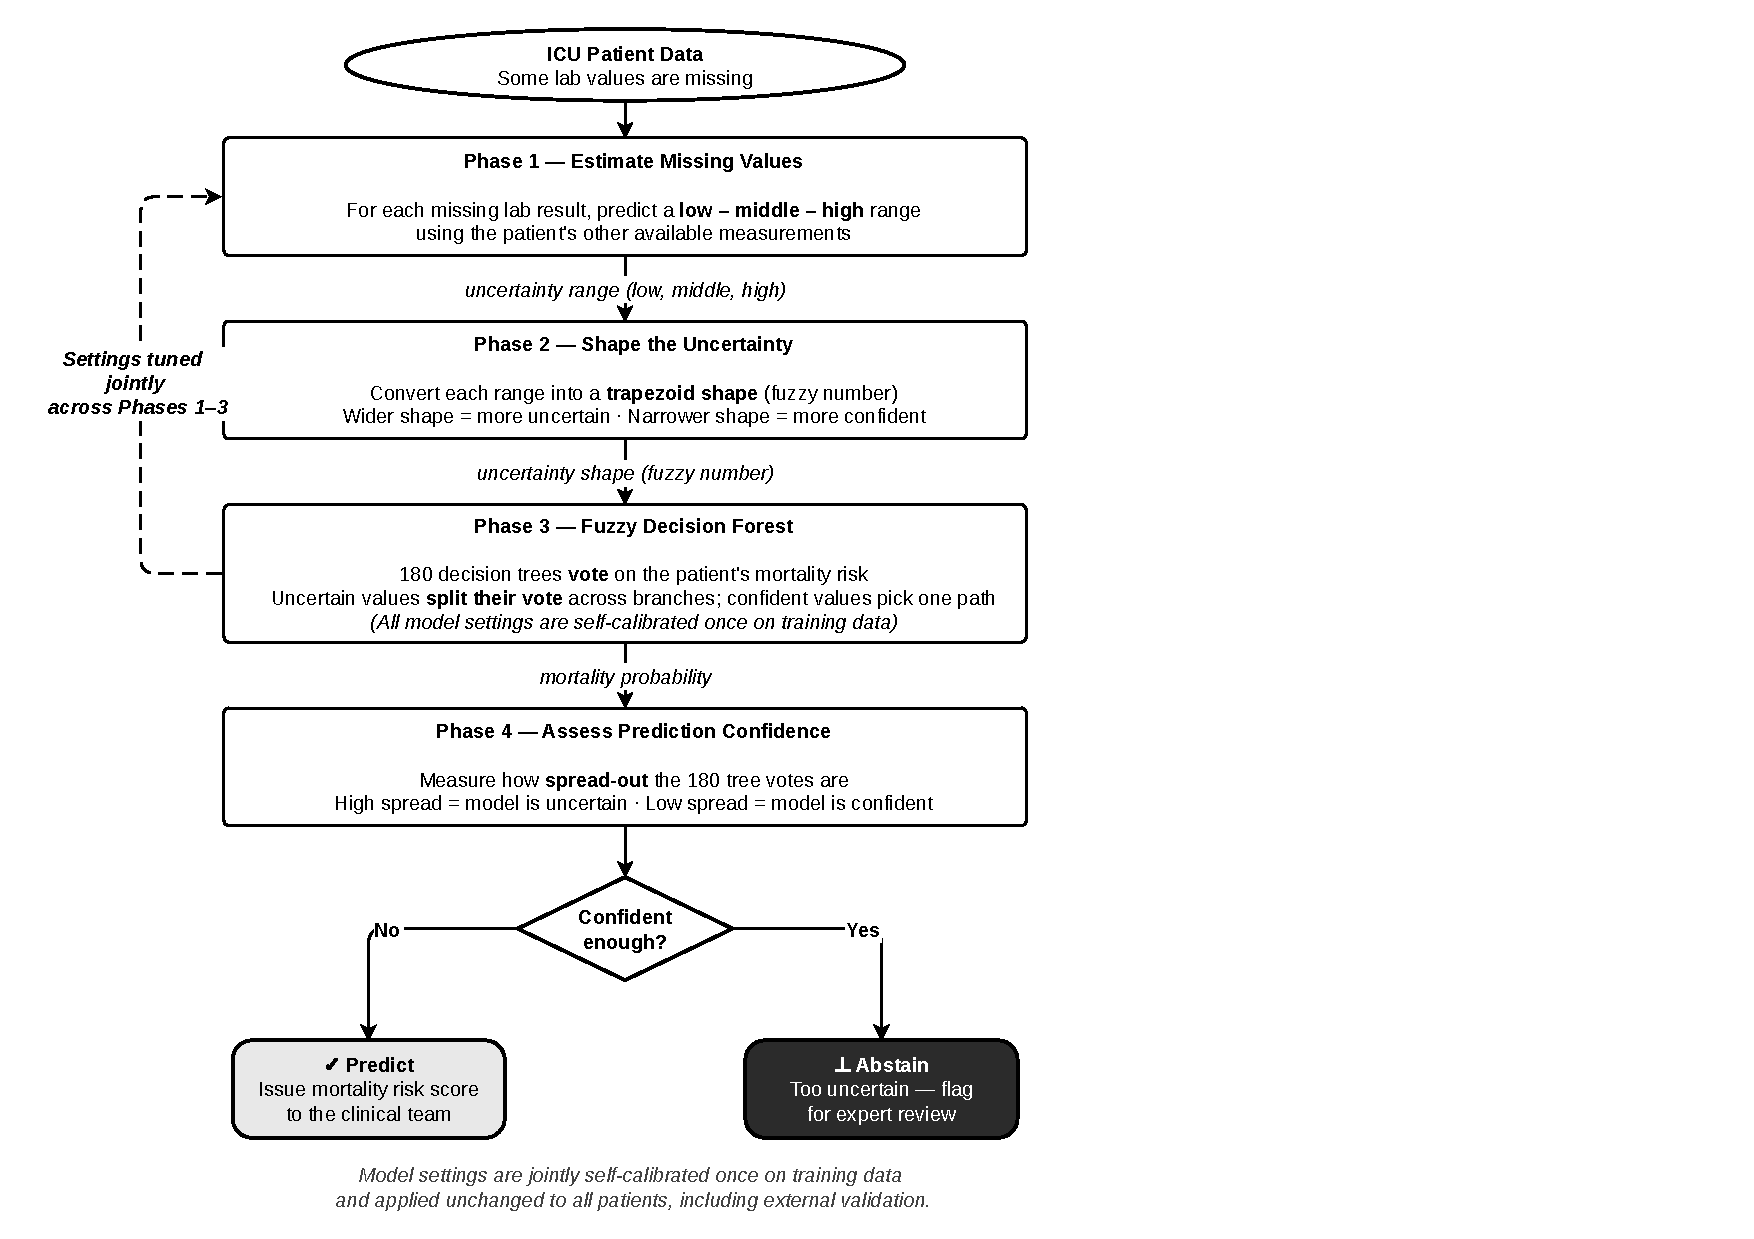
\includegraphics[
	trim=0cm 0cm 9.5cm 0cm, clip=true,
	width=\textwidth,
	height=0.6\textheight, 
	keepaspectratio
	]{fgg1.pdf}
	%\vspace{-70 pt}
	\caption{Overview of the JUCO four-phase pipeline. Phase 1 estimates each missing lab value as a low--middle--high uncertainty range. Phase 2 converts that range into a trapezoid shape whose width encodes uncertainty. Phase 3 routes the patient through 180 decision trees, with uncertain values splitting their vote across branches to produce a mortality probability; settings across Phases 1--3 are jointly calibrated once on training data and applied unchanged thereafter. Phase 4 assesses the spread of those votes: if the model is confident enough it issues a risk score, otherwise it abstains and flags the case for clinical review.}
	\label{fig:architecture}
\end{figure*}

\subsection{Phase 1: Adaptive Quantile Imputation}
\label{sec:phase1}

For each feature $j$ with missing entries, a LightGBM quantile regressor predicts the conditional quantiles of $x_{ij}$ given the remaining observed features $\mathbf{x}_{i,-j}$, minimising the weighted pinball loss

\begin{equation}
	\hat{q}^{\alpha}_{j}(\mathbf{x}_{-j})
	=\arg\min_{f}
	\sum_{i:\,M_{ij}=0}
	w_i\,\rho_{\alpha}\!\left(x_{ij}-f(\mathbf{x}_{i,-j})\right),
	\label{eq:quantile_regression}
\end{equation}

\noindent where $\rho_{\alpha}(u)=u(\alpha-\mathbf{1}_{u<0})$ is the pinball loss~\cite{koenker1978regression} and $w_i$ are the inverse-frequency class weights defined in Appendix~\ref{app:s1}, which give deceased patients roughly ten times the weight of survivors at MIMIC-IV's $\sim$10\% mortality prevalence. Three regressors per feature, at quantile levels $\alpha\in\{\alpha_L,0.5,\alpha_U\}$, yield the triple $(q^L_{ij},q^M_{ij},q^U_{ij})$; $\alpha_L$ and $\alpha_U$ are not fixed but form part of $\boldsymbol{\theta}$, optimised jointly by DE (Section~\ref{sec:de}) rather than committed to a fixed nominal coverage such as 90\% or 95\%. Observed entries pass through unchanged.

\subsection{Phase 2: Proportional Fuzzy Transformation}
\label{sec:phase2}

A wide interval (poorly constrained value) should soften tree routing; a narrow interval should harden it toward crisp behaviour. A trapezoidal fuzzy number~\cite{zimmermann2001fuzzy} satisfies this because its support width $d-a$ is a continuous, monotone function of interval width, a natural carrier for the epistemic uncertainty of Hüllermeier and Waegeman~\cite{hullermeier2021aleatoric}. Each interval is mapped to $\tilde{x}_{ij}=(a_{ij},b_{ij},c_{ij},d_{ij})$ with membership function

\begin{equation}
	\mu_{\tilde{x}_{ij}}(x)=
	\begin{cases}
		0, & x<a_{ij}\text{ or }x>d_{ij},\\[4pt]
		\dfrac{x-a_{ij}}{b_{ij}-a_{ij}}, & a_{ij}\le x<b_{ij},\\[6pt]
		1, & b_{ij}\le x\le c_{ij},\\[4pt]
		\dfrac{d_{ij}-x}{d_{ij}-c_{ij}}, & c_{ij}<x\le d_{ij}.
	\end{cases}
	\label{eq:trapezoid_membership}
\end{equation}

constructed from the quantile outputs as

\begin{align}
	a_{ij} &= q^L_{ij}, \quad
	d_{ij}=q^U_{ij}, \label{eq:fuzzy_a}\\
	b_{ij} &= \max\!\left(a_{ij},\;
	q^M_{ij}-\eta\cdot(q^U_{ij}-q^L_{ij})\right),
	\label{eq:fuzzy_b}\\
	c_{ij} &= \min\!\left(d_{ij},\;
	q^M_{ij}+\eta\cdot(q^U_{ij}-q^L_{ij})\right).
	\label{eq:fuzzy_c}
\end{align}

\noindent where $\eta\in[0,0.5]$ (part of $\boldsymbol{\theta}$) controls the ratio of the flat core $[b,c]$ to the total support $[a,d]$: small $\eta$ gives a wide plateau appropriate under high uncertainty; large $\eta$ approaches a triangular, near-point-imputation shape. Observed entries degenerate to a crisp point ($a=b=c=d=x_{ij}$). Two scalars carry forward to Phase~3 and the DE fitness function:

\begin{align}
	\text{centroid}(\tilde{x}_{ij})
	&=\frac{a_{ij}+b_{ij}+c_{ij}+d_{ij}}{4},
	\label{eq:centroid}\\[4pt]
	\text{uncertainty}(\tilde{x}_{ij})
	&=d_{ij}-a_{ij}.
	\label{eq:uncertainty}
\end{align}

The centroid is the effective feature value for tree routing; it is this uncertainty that drives the sharpness function below.

\begin{figure*}[!t]
	\centering
	%\vspace{-15 pt}
	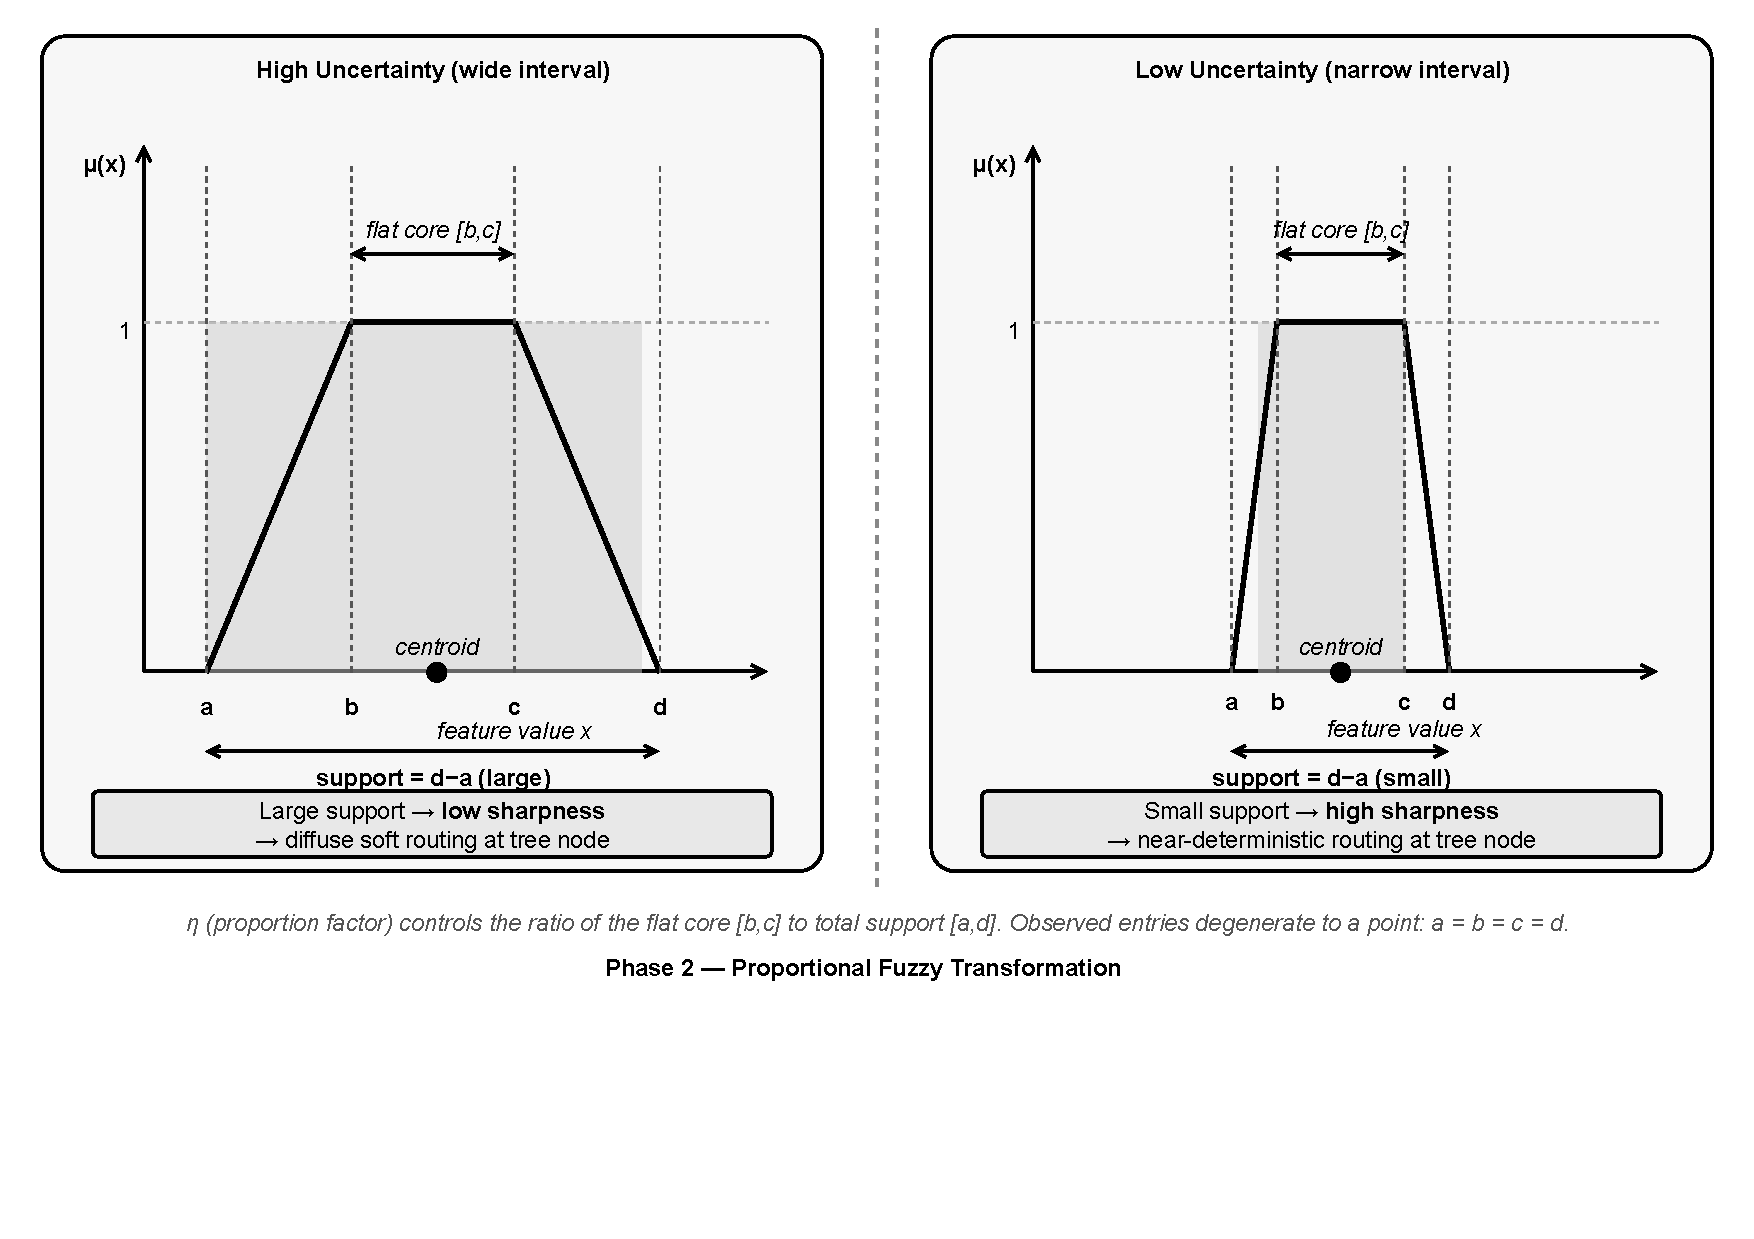
\includegraphics[
	trim=0cm 6cm 0cm 0cm, clip=true,
	width=\textwidth,
	height=0.92\textheight,
	keepaspectratio
	]{fgg2.pdf}
	\vspace{5 pt}
	\caption{Proportional fuzzy transformation (Phase 2). A missing entry with a wide quantile interval (high imputation uncertainty, left panel) produces a broad trapezoidal fuzzy number with large support width $d-a$, resulting in low sharpness and diffuse soft routing at the tree node. A narrow interval (low uncertainty, right panel) produces a nearly-clear trapezoid with small support, which provides high sharpness and nearly-deterministic routing. The centroid serves as an effective feature value for tree routing; the support width is the uncertainty signal passed to the sharpness function. The proportional factor $\eta$ controls the ratio of the flat core $[b,c]$ to the total support $[a,d]$; the observed entries converge to a point: $a=b=c=d$.}
	\label{fig:fuzzy_transformation}
\end{figure*}

\subsection{Phase 3: Fuzzy Decision Forest}
\label{sec:phase3}

Each internal node splits the samples using soft membership degrees instead of a strict binary split. For a node splitting on feature $j$ with triangular fuzzy threshold $\mathcal{T}=(t_{\text{center}},t_{\text{width}})$, the left-child membership $\mu^L_{ij}$ is a sigmoid, $\sigma(z) = 1/(1+e^{-z})$, whose sharpness adapts inversely to combined uncertainty.

\begin{align}
	\text{sharpness}_{ij}
	&=\frac{5}{\text{uncertainty}(\tilde{x}_{ij})+t_{\text{width}}+\varepsilon},
	\label{eq:sharpness}\\[4pt]
	\mu^L_{ij}
	&=\sigma\!\left(\text{sharpness}_{ij}\cdot
	\left(t_{\text{center}}-\text{centroid}(\tilde{x}_{ij})\right)\right),
	\label{eq:mu_left}
\end{align}

\noindent with $\mu^R_{ij}=1-\mu^L_{ij}$ and $\varepsilon=10^{-12}$. Observed inputs ($d_{ij}=a_{ij}$, $t_{\text{width}}\approx0$) drive sharpness toward infinity, producing near-deterministic splits indistinguishable from a crisp tree; imputed inputs with wide intervals produce low sharpness and split their weight across both children, diminishing their leaf influence in proportion to imputation uncertainty. Splits are chosen to maximise fuzzy weighted information gain (fuzzy entropy and gain criteria given in Appendix~\ref{app:s1}), evaluated at seven percentiles of the centroid distribution per candidate feature. At each leaf, the class distribution is formed from the accumulated soft-routed weight vector, so a leaf visited predominantly by imputed samples is more diffuse (and higher-entropy) than one visited predominantly by observed samples, providing the signal Phase~4 converts into abstention.

The forest comprises $K=180$ trees, each trained on a class-balanced bootstrap sample with a fixed random 70\% feature subset per tree; the final prediction averages class probabilities across all trees and is post-hoc isotonic-calibrated~\cite{zadrozny2002transforming} on a held-out set.

\subsubsection{Two-Stage Differential Evolution}
\label{sec:de}

Differential Evolution (DE)~\cite{storn1997differential} jointly optimises $\boldsymbol{\theta}=(\alpha_L,\alpha_U,\eta,d_{\max},n_{\min})$ over the bounded search space $[0.05,0.35]\times[0.65,0.95]\times[0.1,0.5]\times[4,6]\times[15,50]$, suited to this mixed continuous--integer, non-differentiable setting. The composite fitness function is

\begin{equation}
	\mathcal{L}(\boldsymbol{\theta})
	=L_{\text{class}}
	+\lambda_1\cdot\text{MPIW}_{\text{norm}}
	+\lambda_2\cdot\text{coverage\_gap},
	\label{eq:de_fitness}
\end{equation}

\noindent where $L_{\text{class}}$ is the validation log-loss, $\text{MPIW}_{\text{norm}}$ penalises unnecessarily wide imputation intervals, and $\text{coverage\_gap}$ penalises intervals that fail to cover the masked ground-truth values at the nominal target of 95\% (full definition is given in Appendix~\ref{app:s1}); $\lambda_1=0.2$, $\lambda_2=2.0$. The optimization is performed in two stages: the first stage (Stage~1) is a fast global search over a proxy forest ($K=20$ trees, 2,000 points, population 40, $\le12$ generations); the second stage (Stage~2) refines locally around the first-stage optimum ($K=40$ trees, up to 7,000 points, population 60, $\le8$ generations). The resulting $\boldsymbol{\theta}^*$ is obtained once in MIMIC-IV Fold~1 and applied to Folds~2--5 and eICU without any modification, so no test-distribution information enters the optimization loop.

\subsection{Phase 4: Safe Abstention Protocol}
\label{sec:phase4}

Phase~4 converts leaf-level uncertainty into a clinical action using the Shannon entropy of the averaged class probability vector:

\begin{equation}
	H_i=-\sum_{k=0}^{1}\hat{p}_{ik}\log_2(\hat{p}_{ik}+\varepsilon).
	\label{eq:output_entropy}
\end{equation}

Since the imputed samples with wide fuzzy support produce a diffuse leaf distribution (average probability close to 0.5), $H_i$ is systematically higher for patients whose features have many wide-interval imputations, which causally links the omission to the quality of the imputations rather than just the classification margin. The threshold $\tau^*$ is calibrated on the Fold~1 held-out set by minimising $\mathcal{L}(\boldsymbol{\theta}^*)$ over $\tau$ alone; at test time a prediction is issued if $H_i\le\tau^*$ and deferred ($\perp$, flagged for clinician review) otherwise. The frozen threshold from Fold~1 is applied unchanged to Folds~2--5 and to eICU.

	\section{Experimental Setup}
	\label{sec:experimental_setup}
	
	This section describes the datasets, missingness augmentation, cross-validation protocol, calibration, baselines, metrics, and statistical tests used to evaluate JUCO against the problem formalised in Section~\ref{sec:problem_formulation}. Details regarding the computational environment, complexity analysis, and wall-clock runtimes are provided in Appendix~\ref{app:s2}.
	
	\subsection{Datasets}
	\label{sec:datasets}
	
	\textbf{MIMIC-IV} (primary cohort)~\cite{johnson2023mimic}, a single-centre EHR database from Beth Israel Deaconess Medical Center, provides data on 82,785 ICU stays of adult patients (duration: 4 hours to 30 days; data from the first 24 hours were aggregated); following preprocessing, the in-hospital mortality rate is 10.58\%, i.e. imbalanced data. \textbf{eICU} (external validation)~\cite{pollard2018eicu}, 162,136 admissions across 208 US hospitals, was used exclusively for validation: the JUCO parameter vector $\boldsymbol{\theta}^*$ frozen from MIMIC-IV Fold~1 was applied directly, with no retraining, re-optimisation, or threshold recalibration, to test cross-institutional generalisation under genuine distribution shift.
	
	\subsection{Feature Selection}
	\label{sec:feature_selection}
	
	``Mutual information'' between each candidate feature and the mortality-related label is calculated based solely on the training fold; this process retains the top 35 features out of approximately 80 candidates. This conservative threshold primarily reflects the computational cost of the two-stage DE. It does not stem from an assumption that the discarded features lack information (Section~\ref{sec:limitations}).
	
	\subsection{MNAR Augmentation}
	\label{sec:mnar_augmentation}
	
	To evaluate robustness under escalating informative missingness, training and validation folds (not test sets or eICU) receive controlled artificial masking. For observed entry $(i,j)$, the masking probability is
	
	\begin{equation}
		P\!\left(M_{ij}^{\text{aug}}=1\mid x_{ij},\,y_i\right)
		=\sigma\!\left(
		\beta\cdot\frac{x_{ij}-\mu_j}{\sigma_j}
		+\gamma\cdot y_i
		\right).
		\label{eq:mnar_mask}
	\end{equation}
	
	Using the parameters $\beta=-1.0$ (where entries with lower values are preferentially masked, resulting in outcome-correlated missingness) and $\gamma=0.0$ (implying no direct label conditioning), samples were collected iteratively to achieve an overall missingness rate of 30\%, with rates ranging from 10\% to 70\% in the stress-testing experiments.
	
	\subsection{Evaluation Protocol and Calibration}
	\label{sec:evaluation_protocol}
	\label{sec:calibration}
	
	MIMIC-IV uses stratified 5-fold patient-level GroupKFold cross-validation (no patient appears in both train and test); the training fold splits further into train (60\%), validation (20\%, drives DE fitness), and calibration (20\%, drives isotonic calibration~\cite{zadrozny2002transforming} and abstention threshold selection). DE search runs on Fold~1 only; the resulting $\boldsymbol{\theta}^*$ and $\tau^*$ are frozen and applied to Folds~2--5 and eICU without modification, so no test-distribution or eICU information enters optimisation. All models undergo identical isotonic calibration so that ECE/Brier differences reflect model behaviour rather than calibration methodology.
	
	\subsection{Baselines}
	\label{sec:baselines}
	
	Six comparators, evaluated under identical preprocessing and calibration to isolate JUCO's architectural contribution: \textbf{XGBoost}~\cite{chen2016xgboost} and \textbf{LightGBM}~\cite{ke2017lightgbm} (native NaN routing, no imputation); \textbf{MissForest+XGB}~\cite{stekhoven2012missforest} and \textbf{MeanImp+XGB} (point-imputation-then-classify); \textbf{TabNet}~\cite{arik2021tabnet} (attention-based deep learning); and \textbf{JUCO-XGB}, an ablation replacing the fuzzy forest with XGBoost on the same quantile-imputed features, isolating the fuzzy-routing contribution from the imputation contribution.
	
	\subsection{Evaluation Metrics}
	\label{sec:metrics}
	
	AUROC is the primary discrimination metric, with AUPRC (Area Under the Precision-Recall Curve) as a secondary metric more informative under $\sim$10\% mortality prevalence. Expected Calibration Error (ECE, 15 bins)~\cite{naeini2015obtaining} and Brier Score~\cite{brier1950verification} assess calibration (formulas in Appendix~\ref{app:s1}). The Area Under the Risk-Coverage Curve,
	
	\begin{equation}
		\text{AURC}
		=\int_0^1 r(\kappa)\,\mathrm{d}\kappa
		\approx
		\sum_i r_i\cdot\Delta\kappa_i,
		\label{eq:aurc}
	\end{equation}
	
	where $\kappa$ is coverage and $r(\kappa)$ the error rate on the most confident $100\kappa\%$ of predictions, rewards concentrating errors in the abstained region; Risk@90 is the error rate at 90\% coverage. Decision Curve Analysis~\cite{vickers2006decision} computes net benefit
	
	\begin{equation}
		\text{NB}(p_t)
		=\frac{\text{TP}}{n}
		-\frac{p_t}{1-p_t}\cdot\frac{\text{FP}}{n},
		\label{eq:net_benefit}
	\end{equation}
	
	relative to treat-all/treat-none, for $p_t\in[0.01,0.49]$.
	\subsection{Statistical Tests}
	\label{sec:statistical_tests}
	
	Three procedures assess significance transparently: a paired Wilcoxon signed-rank test~\cite{wilcoxon1945individual} on per-fold AUROC (directional only; with 5 folds the minimum achievable two-sided $p$-value is $p=0.0625$, so no comparison reaches formal significance under this test); DeLong's test~\cite{delong1988comparing} on pooled patient-level predictions ($n=82,785$ MIMIC-IV, $n=162,136$ eICU), Bonferroni-corrected to $\alpha=0.0125$; and stratified bootstrap 95\% confidence intervals (1,000 resamples) for AUROC.
	
	\section{Results}
	\label{sec:results}
	
	Results are presented in the following order: robustness under missingness shift, abstention quality, standard-condition comparison, cross-institutional generalisation, decision curve analysis, and a statistical significance summary.
	
	\subsection{Robustness Under Escalating MNAR Missingness}
	\label{sec:stress_results}
	
	\begin{figure}[h]
		\centering
		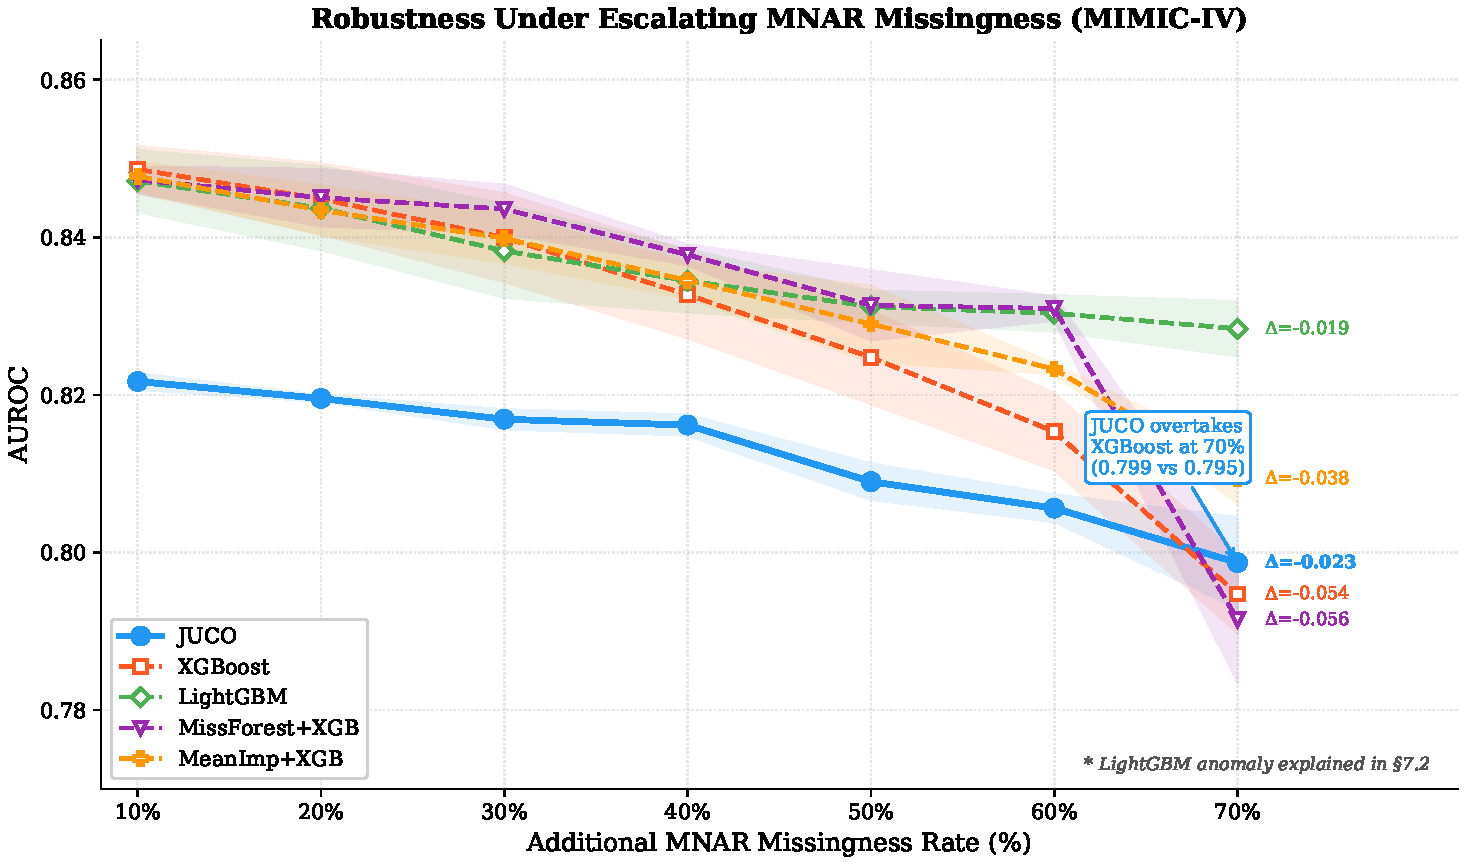
\includegraphics[width=\columnwidth]{Figure4.pdf}
		\caption{AUROC as a function of additional MNAR missingness rate (10\%--70\%) on MIMIC-IV, evaluated on two folds. JUCO's degradation ($-0.023$) is substantially smaller than XGBoost ($-0.054$) and MissForest+XGB ($-0.056$). JUCO outperforms both models in the scenario with 70\% missing data. The anomalous robustness of LightGBM ($-0.019$) is explained methodologically in Section~\ref{sec:lightgbm_anomaly}. Error bars indicate $\pm1$ SD across two evaluation folds.}
		\label{fig:stress_test}
	\end{figure}
	
	Table~\ref{tab:stress_test} presents AUROC across seven MNAR rates. At 10\% missingness, gradient boosting leads (XGBoost 0.849, LightGBM 0.847, MissForest+XGB 0.847, MeanImp+XGB 0.848, versus JUCO 0.822); by 70\%, XGBoost falls to 0.795 ($\Delta=-0.054$), MissForest+XGB to 0.792 ($\Delta=-0.056$), and MeanImp+XGB to 0.809 ($\Delta=-0.038$), while JUCO falls only to 0.799 ($\Delta=-0.023$), numerically overtaking both XGBoost and MissForest+XGB at the most severe rate tested. LightGBM represents an anomalous case ($\Delta=-0.019$, remaining above JUCO throughout); its mechanism is explained in Section~\ref{sec:lightgbm_anomaly}.
	
	\begin{table}[h]
		\centering
		\caption{AUROC under escalating MNAR missingness (MIMIC-IV, two folds, mean $\pm$ SD). Bold indicates the highest AUROC at each rate; $\dagger$ denotes JUCO outperforming gradient boosting at that rate.}
		\label{tab:stress_test}
		\small
		\resizebox{\columnwidth}{!}{%
			\begin{tabular}{lccccccc}
				\toprule
				\textbf{Model} & 10\% & 20\% & 30\% & 40\% & 50\% & 60\% & 70\%\\
				\midrule
				JUCO (Ours) &0.822&0.820&0.817&0.816&0.809&0.806&0.799$^\dagger$\\
				XGBoost &\textbf{0.849}&\textbf{0.845}&0.840&0.833&0.825&0.815&0.795\\
				LightGBM &0.847&0.844&0.838&0.835&\textbf{0.831}&0.830&\textbf{0.828}\\
				MissForest+XGB &0.847&\textbf{0.845}&\textbf{0.844}&\textbf{0.838}&\textbf{0.831}&\textbf{0.831}&0.792$^\dagger$\\
				MeanImp+XGB &0.848&0.843&0.840&0.835&0.829&0.823&0.809\\
				\midrule
				$\Delta$ JUCO &N/A&&$-0.005$&&&&$-0.023$\\
				$\Delta$ XGBoost &N/A&&$-0.009$&&&&$-0.054$\\
				$\Delta$ MissForest &N/A&&$-0.004$&&&&$-0.056$\\
				\bottomrule
		\end{tabular}}
	\end{table}
	
	\subsection{Ablation Study}
	\label{sec:ablation_results}
	
	Table~\ref{tab:ablation} isolates each component's contribution across six variants (two MIMIC-IV folds). The dominant finding is A4 (No Abstention): removing the abstention protocol leaves AUROC, ECE, and Brier Score unchanged while increasing AURC by $2.8\times$ ($0.032\rightarrow0.090$), confirming the entropy signal correctly identifies uncertain predictions rather than withholding indiscriminately. A2 (Crisp Forest) increases ECE by 12.7\% and AURC by 9.4\%, confirming soft routing provides a real calibration benefit. A1 (Sequential optimisation) marginally improves AUROC (0.820 vs.\ 0.818) but worsens AURC, indicating joint optimisation protects risk-coverage behaviour at a small discrimination cost. A3 (Point Imputation) degrades only marginally at standard missingness, with the interval representation's benefit growing under the escalating MNAR conditions of Section~\ref{sec:stress_results}. A5 (No MNAR augmentation) slightly improves in-distribution AUROC but this advantage reverses under escalating missingness, confirming MNAR augmentation is essential for out-of-distribution robustness though unnecessary in-distribution.
	
	\begin{table}[h]
		\centering
		\caption{Ablation study results (MIMIC-IV, two folds, mean $\pm$ SD). Bold indicates the best ablation variant per metric (JUCO Full shown as reference).}
		\label{tab:ablation}
		\small
		\resizebox{\linewidth}{!}{%
			\begin{tabular}{lcccc}
				\toprule
				Variant & AUROC & ECE & Brier & AURC\\
				\midrule
				JUCO (Full) &0.818$\pm$0.001&0.0063$\pm$0.0016&0.072$\pm$0.000&0.0319$\pm$0.0010\\
				A1: Sequential &0.820$\pm$0.003&\textbf{0.0034}$\pm$0.0019&\textbf{0.070}$\pm$0.000&0.0324$\pm$0.0008\\
				A2: Crisp Forest &0.811$\pm$0.004&0.0071$\pm$0.0006&0.071$\pm$0.001&0.0349$\pm$$<0.0001$\\
				A3: Point Impute &0.819$\pm$0.000&0.0053$\pm$0.0012&0.072$\pm$0.001&0.0320$\pm$0.0007\\
				A4: No Abstention &0.818$\pm$0.001&0.0063$\pm$0.0016&0.072$\pm$0.000&0.0895$^\dagger$$\pm$0.0005\\
				A5: No MNAR Aug &\textbf{0.821}$\pm$0.002&0.0043$\pm$0.0010&0.072$\pm$0.000&\textbf{0.0314}$\pm$0.0014\\
				\bottomrule
			\end{tabular}
		}
		\smallskip
		\raggedright\footnotesize
		$^\dagger$A4 makes no abstentions; the risk-coverage curve is flat at the full-coverage error rate, so AURC $=1-\text{Accuracy}\approx0.091$. ECE values for JUCO Full and A4 are reported from the 5-fold main evaluation (Table~\ref{tab:main_results}) for consistency; the 2-fold ablation run yields ECE $= 0.0049$ for both variants.
	\end{table}
	
	\begin{figure}[h]
		\centering
		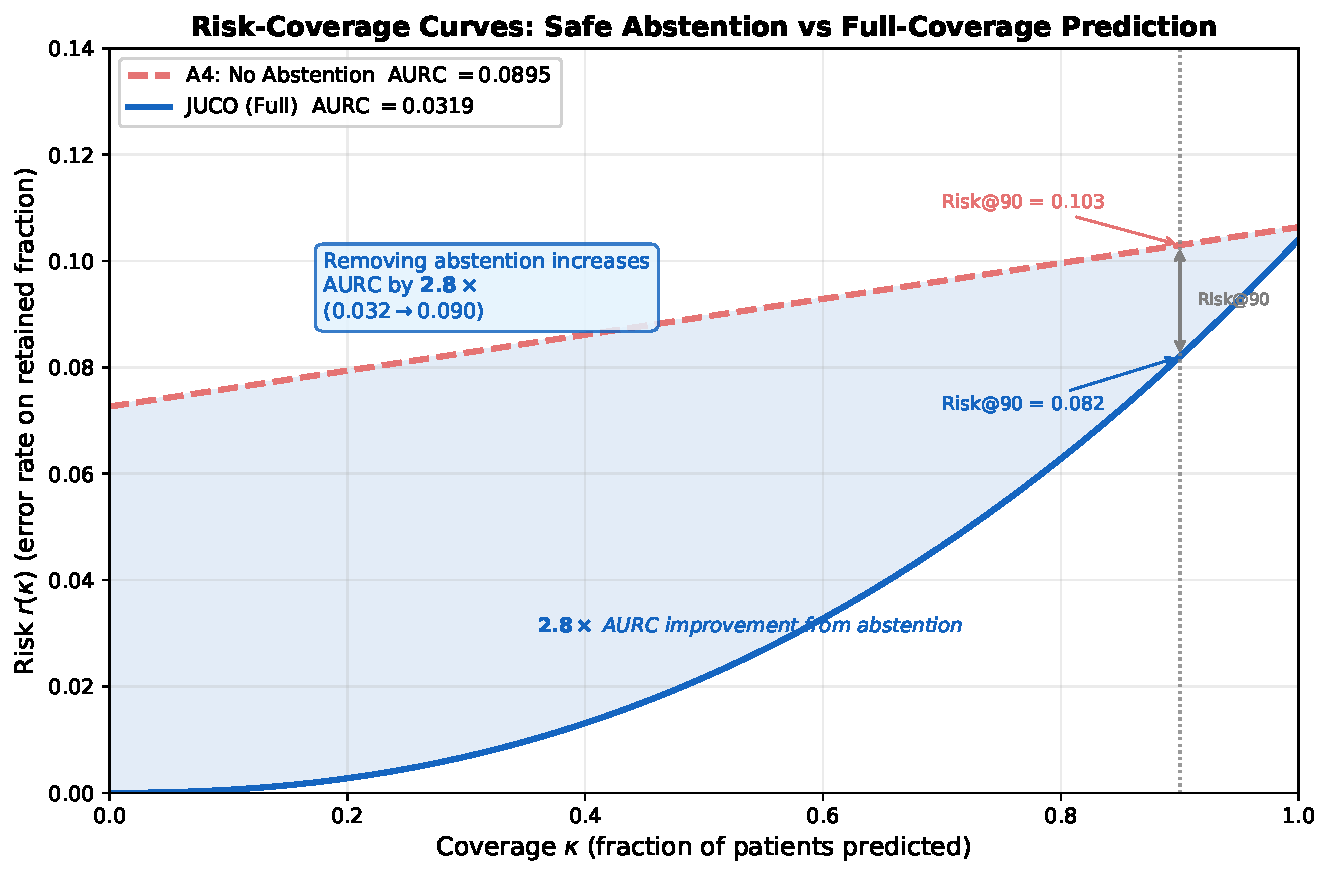
\includegraphics[width=\columnwidth]{Figure5.pdf}
		\caption{Risk-coverage curves on MIMIC-IV for JUCO (Full) and A4 (No Abstention). JUCO Full achieves AURC $=0.032$ versus A4's $0.090$ ($2.8\times$ increase without abstention). The largest separation occurs at low coverage, indicating that abstention primarily protects the most uncertain patients. Risk@90 is also substantially lower for JUCO Full.}
		\label{fig:risk_coverage}
	\end{figure}
	
	\begin{table*}[htbp]
		\centering
		\caption{Main results on MIMIC-IV (5-fold cross-validation, mean $\pm$ SD). Bold indicates the best value per metric.}
		\label{tab:main_results}
		\small
		\begin{tabular}{lccccccc}
			\toprule
			Model & AUROC & AUPRC & ECE & Brier & AURC & Risk@90 & F1\\
			\midrule
			JUCO (Ours)&0.814$\pm$0.003&0.453$\pm$0.007&0.0063$\pm$0.0016&0.074$\pm$0.002&0.034$\pm$0.002&0.065$\pm$0.002&0.651$\pm$0.014\\
			XGBoost$^\ddagger$&\textbf{0.842}$\pm$0.004&0.511$\pm$0.010&0.0065$\pm$0.0027&\textbf{0.069}$\pm$0.001&\textbf{0.028}$\pm$0.001&\textbf{0.059}$\pm$0.001&0.674$\pm$0.012\\
			LightGBM$^\ddagger$&0.842$\pm$0.003&\textbf{0.515}$\pm$0.009&0.0065$\pm$0.0020&\textbf{0.069}$\pm$0.001&\textbf{0.028}$\pm$0.001&\textbf{0.059}$\pm$0.001&0.674$\pm$0.008\\
			MissForest+XGB$^\ddagger$&\textbf{0.843}$\pm$0.002&0.514$\pm$0.008&\textbf{0.0060}$\pm$0.0015&\textbf{0.069}$\pm$0.001&\textbf{0.028}$\pm$0.001&\textbf{0.058}$\pm$0.002&\textbf{0.681}$\pm$0.018\\
			MeanImp+XGB&0.842$\pm$0.004&N/A&0.0063$\pm$0.0025&\textbf{0.069}$\pm$0.001&\textbf{0.028}$\pm$0.001&\textbf{0.059}$\pm$0.001&\textbf{0.681}$\pm$0.004\\
			JUCO-XGB$^\S$&0.770$\pm$0.002&0.269$\pm$0.009&0.0075$\pm$0.0020&0.084$\pm$0.002&0.041$\pm$0.001&0.085$\pm$0.002&0.522$\pm$0.010\\
			TabNet (DL)$^{\ddagger\ddagger}$&0.738$\pm$0.086&N/A&0.0609$\pm$0.1067&0.121$\pm$0.084&0.096$\pm$0.108&0.142$\pm$0.141&0.574$\pm$0.073\\
			\bottomrule
		\end{tabular}
		
		\smallskip
		\raggedright\footnotesize
		DeLong tests: JUCO vs XGBoost ($z=-18.04$, $p<0.001$), JUCO vs LightGBM ($z=-16.45$, $p<0.001$), JUCO vs MissForest ($z=-19.20$, $p<0.001$), and JUCO vs JUCO-XGB ($z=+22.04$, $p<0.001$).
		
		\smallskip
		$^{\ddagger\ddagger}$TabNet Fold~1 AUROC $=0.567$ indicates convergence failure on CPU hardware; excluded from primary comparisons. $^{\S}$JUCO-XGB MIMIC-IV results sourced from a separate robustness experiment script; eICU results from a separate external-validation script. MeanImp+XGB and TabNet AUPRC not available.
	\end{table*}
	
	\subsection{Baseline Comparison Under Standard 30\% MNAR}
	\label{sec:baseline_results}
	
	Under standard 30\% MNAR conditions, gradient boosting retains a statistically significant AUROC advantage over JUCO, reported here transparently and explained mechanistically in Section~\ref{sec:auroc_gap}. Table~\ref{tab:main_results} presents the full seven-metric comparison. The gap is significant across all three baselines (DeLong $z=-16.45$ to $-19.20$, $p<0.001$), while JUCO significantly outperforms its own JUCO-XGB ablation ($z=+22.04$, $p<0.001$; AUROC 0.814 vs.\ 0.770), confirming the fuzzy forest adds real value beyond interval-valued imputation alone. Post-hoc calibration brings JUCO's ECE (0.0063) to a level comparable with gradient boosting (0.0060--0.0065) despite lower AUROC. Gradient boosting achieves lower AURC under standard conditions (0.028 vs.\ JUCO's 0.034), but this conflates a lower full-coverage error rate with JUCO's additional capability: a principled abstention mechanism enabling selective deployment at any point on the risk-coverage curve.
	
	
	
	\subsection{External Validation on eICU}
	\label{sec:eicu_results}
	
	Table~\ref{tab:eicu_results} presents results on eICU using parameters frozen from MIMIC-IV Fold~1, the strongest evidence for JUCO's primary claim. The AUROC gap between JUCO and XGBoost contracts by 46\% ($-0.028$ on MIMIC-IV to $-0.015$ on eICU), consistent with gradient boosting's NaN-routing advantage diminishing under genuine cross-institutional shift. JUCO's ECE on eICU (0.0029) is lower than on MIMIC-IV (0.0063) despite frozen isotonic parameters fitted on MIMIC-IV alone, confirming the calibration improvement arises from the representation itself rather than recalibration; AURC on eICU (0.016) reaches near-parity with XGBoost (0.016).
	
	\begin{table}[h]
		\centering
		\caption{External validation on eICU (208 hospitals, frozen parameters, mean $\pm$ SD).}
		\label{tab:eicu_results}
		\small
		\resizebox{\linewidth}{!}{%
			\begin{tabular}{lcccc}
				\toprule
				Model & AUROC & ECE & AURC & NB@0.10\\
				\midrule
				JUCO (Ours)&0.819$\pm$0.005&0.0029$\pm$0.0009&0.016$\pm$0.001&0.020$\pm$0.002\\
				XGBoost&\textbf{0.834}$\pm$0.005&0.0030$\pm$0.0012&\textbf{0.016}$\pm$0.001&\textbf{0.021}$\pm$0.002\\
				LightGBM&0.831$\pm$0.005&0.0026$\pm$0.0011&0.016$\pm$0.001&0.021$\pm$0.002\\
				MissForest+XGB&0.833$\pm$0.004&\textbf{0.0024}$\pm$0.0011&0.016$\pm$0.001&0.021$\pm$0.002\\
				\bottomrule
			\end{tabular}
		}
	\end{table}
	
	\subsection{Decision Curve Analysis}
	\label{sec:dca_results}
	
	Table~\ref{tab:dca} shows all models provide positive net benefit relative to treat-all/treat-none across the threshold range. On MIMIC-IV, JUCO's net benefit trails gradient boosting at all thresholds; on eICU, this gap narrows at every threshold, mirroring the AUROC gap reduction in Table~\ref{tab:eicu_results}.
	
	\begin{table}[h]
		\centering
		\caption{Net benefit at key clinical decision thresholds.}
		\label{tab:dca}
		\small
		\resizebox{\linewidth}{!}{%
			\begin{tabular}{lcccccc}
				\toprule
				&\multicolumn{3}{c}{MIMIC-IV}&\multicolumn{3}{c}{eICU}\\
				\cmidrule(lr){2-4}\cmidrule(lr){5-7}
				Model&0.05&0.10&0.20&0.05&0.10&0.20\\
				\midrule
				JUCO&0.069&0.049&0.032&0.026&0.020&0.014\\
				XGBoost&0.071&0.054&0.036&0.027&0.021&0.015\\
				LightGBM&0.072&0.054&0.036&0.027&0.021&0.015\\
				MissForest+XGB&0.072&0.055&0.037&0.028&0.021&0.016\\
				Treat all&0.057&0.004&N/A&0.004&N/A&N/A\\
				Treat none&0&0&0&0&0&0\\
				\bottomrule
			\end{tabular}
		}
	\end{table}
	
	\vspace{0 pt}
	\begin{figure}[h]
		\centering
		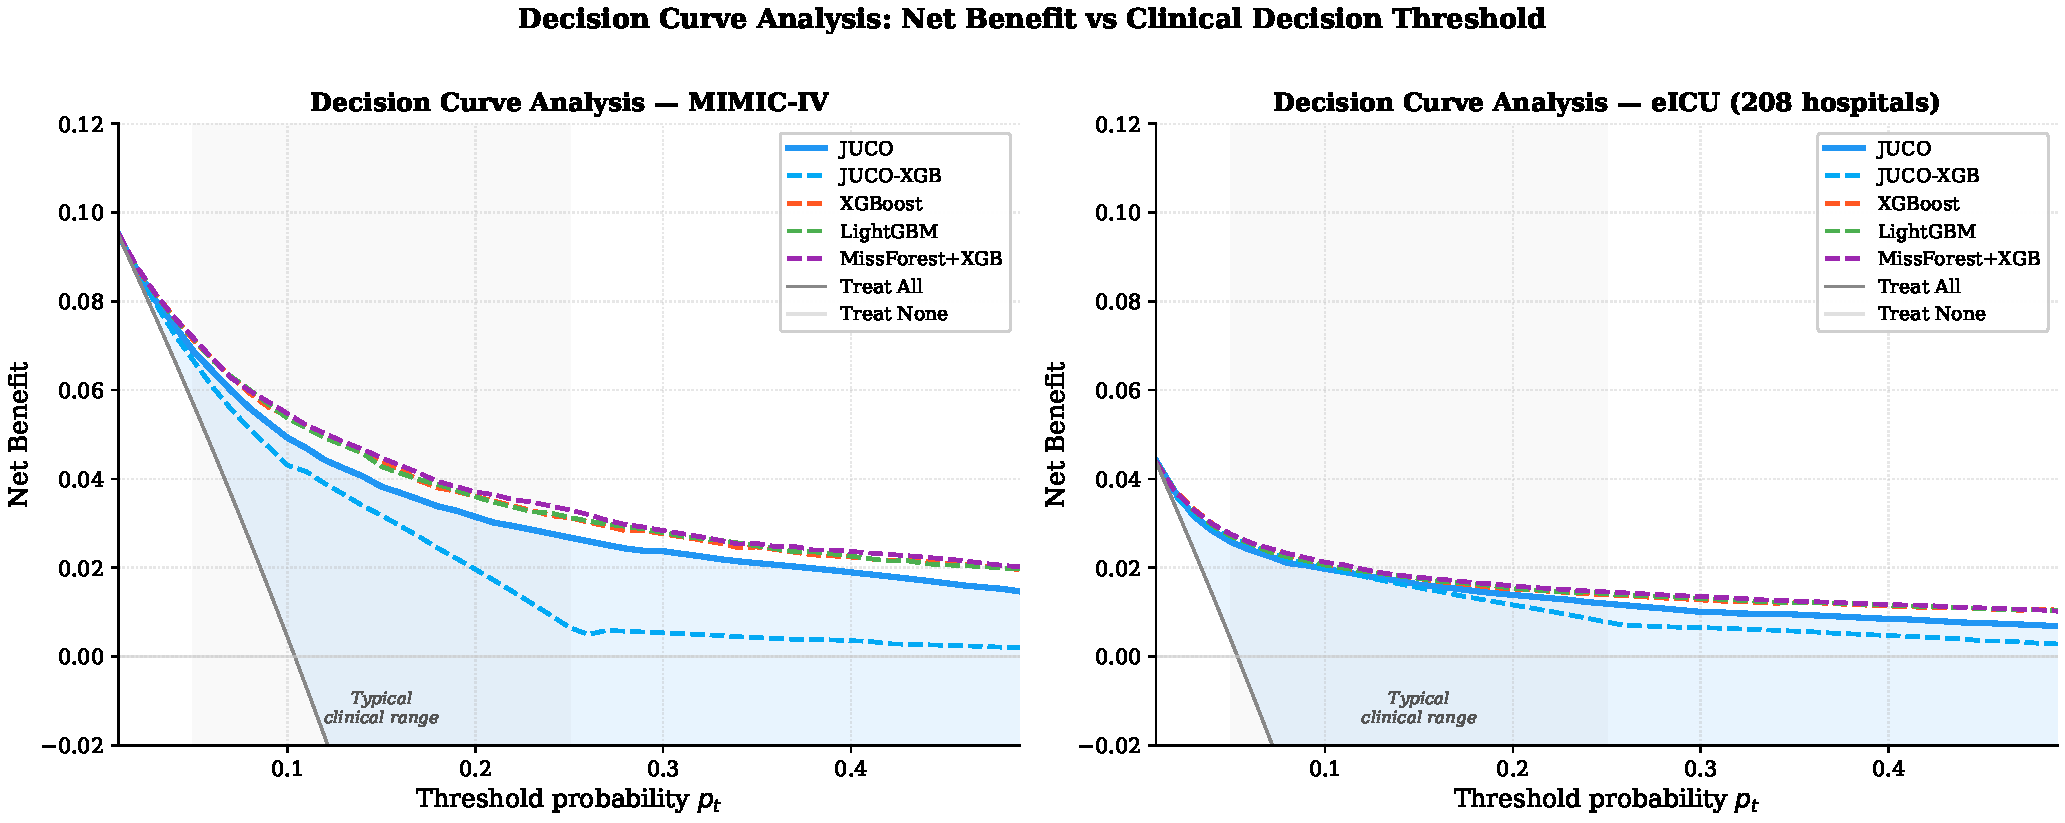
\includegraphics[width=\columnwidth]{Figure6.pdf}
		\caption{Decision curve analysis on MIMIC-IV (left) and eICU (right). All models outperform treat-all and treat-none baselines; JUCO's gap narrows under external validation.}
		\label{fig:dca}
	\end{figure}
	
	\subsection{Statistical Significance Summary}
	\label{sec:stat_summary}
	
	Table~\ref{tab:delong} consolidates DeLong test results across both datasets. The magnitude of the test statistic falls substantially from MIMIC-IV to eICU for every comparison against gradient boosting (XGBoost: $-18.04\rightarrow-9.88$; LightGBM: $-16.45\rightarrow-7.62$; MissForest: $-19.20\rightarrow-9.56$), confirming that the gap contraction reported in Section~\ref{sec:eicu_results} is a systematic property of cross-institutional transfer rather than an artefact of eICU's different class prevalence. JUCO's significant advantage over JUCO-XGB persists on both datasets ($z=+22.04$ on MIMIC-IV, $z=+2.86$ on eICU), confirming the fuzzy forest's contribution is not specific to the training institution.
	
	\begin{table}[h]
		\centering
		\caption{DeLong test results for JUCO versus baselines.}
		\label{tab:delong}
		
		\resizebox{\linewidth}{!}{%
			\begin{tabular}{llccl}
				\toprule
				Dataset&Comparison&$z$&$p$&Direction\\
				\midrule
				MIMIC-IV&JUCO vs XGBoost&$-18.04$&$<0.001$&XGBoost superior\\
				MIMIC-IV&JUCO vs LightGBM&$-16.45$&$<0.001$&LightGBM superior\\
				MIMIC-IV&JUCO vs MissForest&$-19.20$&$<0.001$&MissForest superior\\
				MIMIC-IV&JUCO vs JUCO-XGB&$+22.04$&$<0.001$&JUCO superior\\
				eICU&JUCO vs XGBoost&$-9.88$&$<0.001$&XGBoost superior (gap narrowed)\\
				eICU&JUCO vs LightGBM&$-7.62$&$<0.001$&LightGBM superior (gap narrowed)\\
				eICU&JUCO vs MissForest&$-9.56$&$<0.001$&MissForest superior (gap narrowed)\\
				eICU&JUCO vs JUCO-XGB&$+2.86$&0.004&JUCO superior\\
				\bottomrule
			\end{tabular}
		}
	\end{table}
	
	
	\section{Discussion}
	\label{sec:discussion}
	
	\label{sec:auroc_gap}
	The results reveal a consistent trade-off that resolves the apparent contradiction between JUCO's lower nominal AUROC under standard conditions and its stronger behaviour under deployment-relevant shifts. Under conventional 30\% MNAR conditions, gradient boosting achieves the highest discrimination (AUROC 0.842--0.843 versus JUCO's 0.814), and DeLong's test confirms this difference is statistically significant (Table~\ref{tab:delong}). However, this advantage contracts substantially when the missingness mechanism changes: under escalating MNAR stress, JUCO's degradation is less than half that of XGBoost ($-0.023$ versus $-0.054$), and during genuine cross-institutional validation on eICU the AUROC gap contracts by 46\% ($-0.028 \rightarrow -0.015$). The implication is that gradient boosting extracts more performance from a stationary missingness proxy, whereas JUCO sacrifices some of that proxy-dependent advantage in exchange for substantially greater robustness once the missingness mechanism changes.
	
	This interpretation is reinforced by the ablation study. Removing fuzzy routing (A2) degrades calibration while leaving discrimination relatively intact, indicating that the fuzzy representation primarily improves probability quality rather than ranking ability. Removing abstention (A4) leaves AUROC unchanged but increases AURC by $2.8\times$, confirming that entropy-based rejection concentrates errors in precisely the patients whose imputation uncertainty is greatest. Meanwhile, replacing the fuzzy forest with XGBoost on identical quantile-imputed features (JUCO-XGB) reduces AUROC from 0.814 to 0.770, demonstrating that interval-valued imputation alone is insufficient and that uncertainty must continue influencing downstream routing.
	
	A second noteworthy observation concerns calibration. JUCO's ECE improves from 0.0063 on MIMIC-IV to 0.0029 on eICU despite using the same frozen isotonic calibration learned on MIMIC-IV alone. Since no recalibration occurs on eICU, this improvement cannot be attributed to post-processing; instead, it suggests that propagating imputation uncertainty structurally produces probability estimates that remain well behaved even after institutional shift. This behaviour contrasts with approaches that rely on NaN routing, where the missingness pattern itself becomes institution-specific.
	
	\label{sec:lightgbm_anomaly}
	The remaining anomaly is LightGBM. Unlike XGBoost, LightGBM degrades only by $-0.019$ under synthetic MNAR stress and remains numerically above JUCO throughout Figure~\ref{fig:stress_test}. This does not contradict the central claim because the stress test modifies only additional missingness while preserving the original feature distribution; LightGBM's histogram-based split construction appears unusually resistant under this restricted perturbation. Yet under the real cross-institutional shift represented by eICU, LightGBM's advantage contracts alongside XGBoost's, supporting the broader conclusion that synthetic robustness and deployment robustness are not equivalent.
	
	Taken together, these findings suggest that ICU mortality prediction should not be evaluated solely by discrimination under a fixed missingness pattern. A model that preserves calibration, identifies unreliable predictions, and degrades gradually when documentation behaviour changes may provide greater practical value than one whose highest AUROC depends on institutional missingness conventions remaining unchanged.
	
	\subsection{Limitations}
	\label{sec:limitations}
	
	Several limitations qualify these findings. JUCO uses only the first 24 hours of structured ICU data, omitting temporal trajectories, clinical notes, imaging, and waveform signals that may carry additional prognostic value. Feature selection retains only the top 35 variables, a threshold driven by the computational cost of two-stage Differential Evolution rather than the informativeness of the excluded features, so this remains a practical bottleneck for larger feature spaces. The fuzzy decision forest is also more expensive to train than conventional gradient boosting, though inference speed remains clinically practical. The synthetic MNAR mechanism used for stress testing is a controlled logistic masking process rather than a full reproduction of hospital-specific documentation behaviour; the eICU validation demonstrates genuine institutional transferability, but further prospective evaluation would strengthen this evidence. Finally, abstention was evaluated retrospectively, and future studies should examine how clinicians respond to deferred cases within real decision-support workflows.
	
	\section{Conclusion and Future Work}
	\label{sec:conclusion}
	
	This work introduced JUCO, a joint uncertainty-calibrated framework for ICU mortality prediction that propagates imputation uncertainty through quantile intervals, fuzzy representations, soft-routing decision forests, and entropy-based abstention instead of collapsing uncertainty before classification. The principal finding is not that JUCO achieves the highest conventional AUROC (it does not) but that its performance degrades substantially more slowly as informative missingness increases and that its cross-institutional performance contracts far less than competing approaches when evaluated with frozen parameters on eICU. The combination of uncertainty propagation and selective abstention produces calibrated predictions while explicitly identifying patients whose predictions are least trustworthy, yielding a $2.8\times$ improvement in selective reliability (AURC) without requiring institution-specific retraining. Rather than eliminating imputation uncertainty prior to classification, propagating it structurally through the prediction pipeline yields a model that, despite a slight performance trade-off under stable conditions, offers significantly greater robustness against missingness shifts and across-institution deployment; this is precisely the context where clinical decision support is most needed yet least proven to be reliable. Future work will extend this framework beyond the first 24 hours of structured data to incorporate temporal trajectories and clinical text, evaluate abstention prospectively within live clinical workflows, and test robustness under more realistic, multi-directional missingness mechanisms than the controlled logistic masking used here.
	
	\appendices
	
	\section{Auxiliary Equations and Derivations}
	\label{app:s1}
	
	\subsection{Inverse-Frequency Class Weights (Phase 1)}
	
	The pinball-loss quantile regressors in Phase~1 (Eq.~\ref{eq:quantile_regression}) are trained with inverse-frequency sample weights to correct for class imbalance at the imputation stage. The weight assigned to each sample from class $k$ is
	\begin{equation}
		w_k = \frac{N}{K \cdot n_k},
		\label{eq:class_weights}
	\end{equation}
	where $N$ is the total number of training samples, $K=2$ is the number of classes, and $n_k$ is the count of class-$k$ samples. At the approximately 10\% mortality prevalence observed in MIMIC-IV ($n_1 \approx 0.1N$), deceased patients receive approximately ten times the weight of surviving patients, ensuring the quantile regressors are fitted with equal aggregate influence from both outcome classes rather than being dominated by the survivor majority.
	
	\subsection{Fuzzy Weighted Entropy and Split Criterion (Phase 3)}
	
	Splits in the fuzzy decision forest (Section~IV-C) are chosen to maximise fuzzy weighted information gain. The fuzzy weighted entropy at a node with accumulated sample weight vector $\mathbf{w}$ is
	\begin{equation}
		H_{\text{fuzzy}}(\mathbf{w}, \mathbf{y})
		= -\sum_{k=0}^{1}
		\tilde{p}_k \log_2(\tilde{p}_k + \varepsilon),
		\quad
		\tilde{p}_k =
		\frac{\sum_{i:\, y_i = k} w_i}{\sum_i w_i + \varepsilon},
		\label{eq:fuzzy_entropy}
	\end{equation}
	and the fuzzy information gain for a candidate split is
\begin{equation}
	\begin{split}
		\Delta H &= H_{\text{fuzzy}}(\mathbf{w},\,\mathbf{y})
		-\frac{\sum_i w_i\mu^L_i}{\sum_i w_i}
		H_{\text{fuzzy}}(\mathbf{w}\circ\boldsymbol{\mu}^L,\,\mathbf{y}) \\
		&\quad
		-\frac{\sum_i w_i\mu^R_i}{\sum_i w_i}
		H_{\text{fuzzy}}(\mathbf{w}\circ\boldsymbol{\mu}^R,\,\mathbf{y}),
	\end{split}
	\label{eq:fuzzy_gain}
\end{equation}
	where $\circ$ denotes elementwise multiplication and $\mu^L_i, \mu^R_i$ are the left/right soft-routing membership degrees defined in Eq.~\ref{eq:mu_left}. Split thresholds are evaluated at the $\{15, 30, 45, 50, 55, 70, 85\}$ percentiles of the centroid distribution for each candidate feature.
	
	At each leaf node, the class distribution is formed from the accumulated soft-routed weight vector $\mathbf{w}_\ell$:
	\begin{equation}
		\hat{p}^{\ell}_k
		= \frac{\sum_{i:\, y_i = k} w^\ell_i}
		{\sum_i w^\ell_i + \varepsilon},
		\quad k \in \{0, 1\}.
		\label{eq:leaf_dist}
	\end{equation}
	The final forest prediction for patient $i$ averages class probabilities across all $K=180$ trees:
	\begin{equation}
		\hat{\mathbf{p}}_i =
		\frac{1}{K} \sum_{k=1}^{K} \hat{\mathbf{p}}^{(k)}_i.
		\label{eq:forest_avg}
	\end{equation}
	
	\subsection{DE Fitness Function Components}
	
	The composite Differential Evolution fitness function (Eq.~\ref{eq:de_fitness}) is
	
		\[
	\mathcal{L}(\boldsymbol{\theta}) =
	L_{\text{class}}
	+ \lambda_1 \cdot \text{MPIW}_{\text{norm}}
	+ \lambda_2 \cdot \text{coverage\_gap},
	\]
	
	where $\lambda_1=0.2$ and $\lambda_2=2.0$.
	The normalised Mean Prediction Interval Width term penalises unnecessarily wide imputation intervals:
	\begin{equation}
		\text{MPIW}_{\text{norm}} =
		\frac{1}{d} \sum_{j=1}^{d}
		\frac{|q^U_j - q^L_j|}
		{\max_j - \min_j + \varepsilon}.
		\label{eq:mpiw}
	\end{equation}
	The coverage-gap term penalises intervals that fail to cover the true imputed values at the nominal 95\% target level:
	\begin{equation}
		\text{coverage\_gap} =
		\max\!\left(0,\; 0.95 - \widehat{\text{PICP}}\right),
		\label{eq:coverage_gap}
	\end{equation}
	where the Prediction Interval Coverage Probability is
	\begin{equation}
		\widehat{\text{PICP}} =
		\frac{1}{|\mathcal{I}|}
		\sum_{(i,j) \in \mathcal{I}}
		\mathbf{1}\!\left[q^L_{ij} \le x^{\text{true}}_{ij}
		\le q^U_{ij}\right],
		\label{eq:picp}
	\end{equation}
	with $\mathcal{I}$ the set of artificially masked entries for which the ground-truth value is available.
	
	\subsection{Differential Evolution Configuration}
	
	Table~\ref{tab:de_config_supp} summarises the DE configuration used for both stages of the two-stage optimisation (Section~IV-C1).
	
	\begin{table}[h]
		\centering
		\caption{Differential Evolution configuration.}
		\label{tab:de_config_supp}
		\begin{tabular}{lll}
			\toprule
			\textbf{Parameter} & \textbf{Stage 1 (coarse)} & \textbf{Stage 2 (fine)} \\
			\midrule
			Strategy & best1bin & best1bin \\
			Population size ($\times d$) & 8$\times$5 & 12$\times$5 \\
			Max iterations & 8 & 12 \\
			Mutation ($F$) & 0.5--1.0 (dithered) & 0.5--1.0 (dithered) \\
			Crossover ($CR$) & 0.7 & 0.7 \\
			Convergence tol. & $10^{-4}$ & $10^{-4}$ \\
			Proxy forest size & 20 trees & 40 trees \\
			Proxy data cap & 2{,}000 samples & 7{,}000 samples \\
			Early stopping (patience) & 3 generations & 3 generations \\
			Polishing (L-BFGS-B) & disabled & disabled \\
			Population updating & deferred & deferred \\
			\bottomrule
		\end{tabular}
	\end{table}
	
	Stage~2 seeds its initial population around the Stage-1 optimum with $\pm15\%$ of each parameter's range, enabling rapid local refinement without escaping the vicinity of the global optimum found in Stage~1. Both stages use patience-based early stopping of 3 generations without improvement to avoid unnecessary fitness evaluations once the population has converged; L-BFGS-B polishing is disabled (\texttt{polish=False}) to keep the solution within the discrete-compatible parameter space; and population updates are deferred (\texttt{updating="deferred"}) so that all fitness evaluations within a generation complete before any individual is replaced, ensuring reproducible parallel-safe behaviour across the 12 DE workers.
	
	\subsection{Evaluation Protocol Schematic}
	
	Figure~\ref{fig:eval_protocol_supp} illustrates the cross-validation and parameter-freezing protocol applied throughout this study, referenced from Section~V-D.
	
	\begin{figure*}[h]
		\centering
		%\vspace{-10pt}
		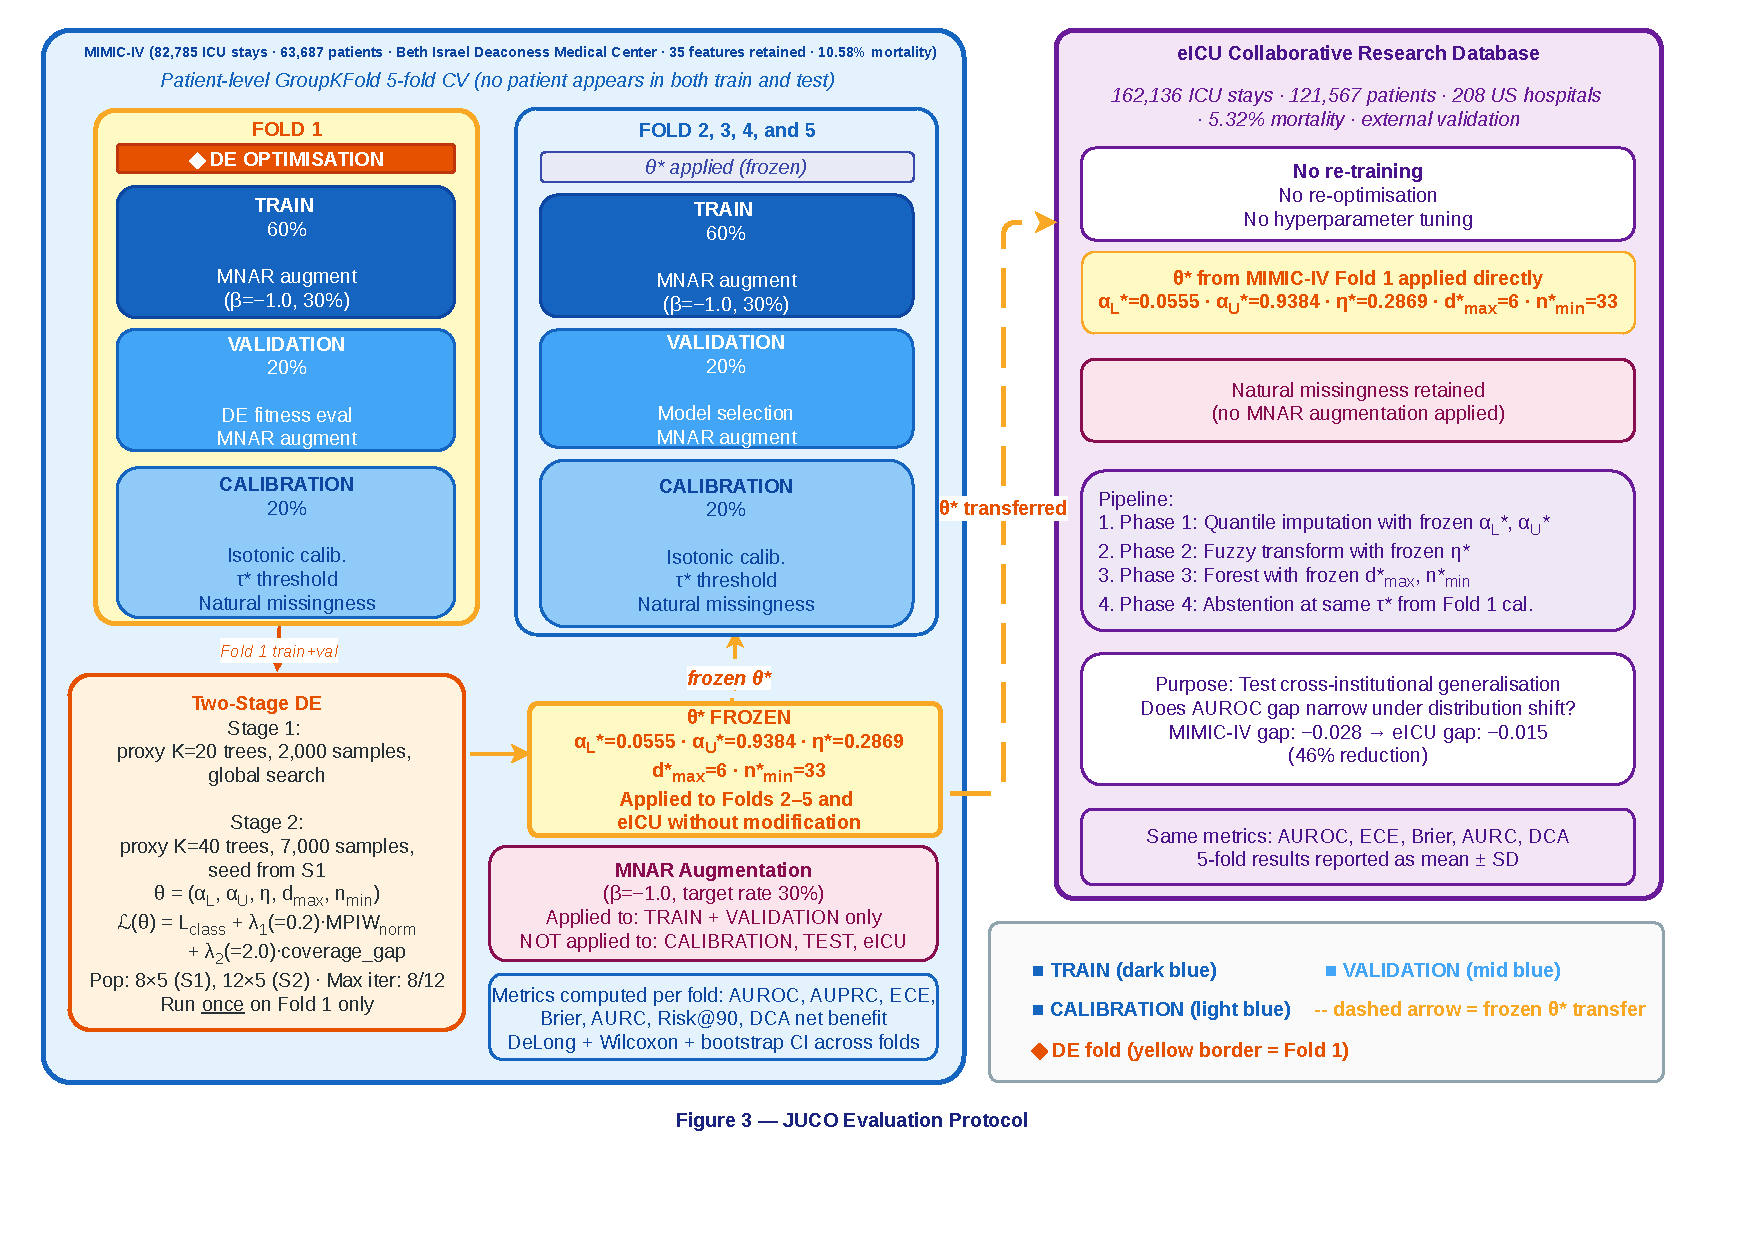
\includegraphics[
		trim=0cm 2.5cm 1cm 0cm, clip=true,
		width=\textwidth,
		height=0.9\textheight,keepaspectratio]{fgg3.pdf}
		\vspace{5 pt}
		\caption{Evaluation protocol. MIMIC-IV is partitioned using patient-level GroupKFold 5-fold cross-validation to prevent data leakage. Each training fold is further divided into train, validation, and calibration subsets. DE hyperparameter search runs once on Fold~1; the resulting $\boldsymbol{\theta}^*$ is frozen and applied unchanged to Folds~2--5 and the eICU external validation set. MNAR augmentation (Eq.~\ref{eq:mnar_mask}) is applied only to training and validation subsets.}
		\label{fig:eval_protocol_supp}
	\end{figure*}
	
	\subsection{Calibration and Selective-Prediction Metric Formulas}
	
	Expected Calibration Error (ECE), 15 equal-width bins:
	\begin{equation}
		\text{ECE} = \sum_{b=1}^{B} \frac{n_b}{N}
		\left|\overline{p}_b - \text{freq}_b\right|,
		\quad B = 15,
		\label{eq:ece}
	\end{equation}
	where $\overline{p}_b$ is the mean predicted probability in bin $b$, $\text{freq}_b$ is the fraction of positive outcomes in that bin, $n_b$ is the number of samples in bin $b$, and $N$ is the total number of samples.
	
	Brier Score:
	\begin{equation}
		\text{BS} = \frac{1}{n}
		\sum_{i=1}^{n}(\hat{p}_i - y_i)^2.
		\label{eq:brier}
	\end{equation}
	
	\section{Computational Environment, Complexity, and Runtimes}
	\label{app:s2}
	
	\subsection{Hardware and Software}
	
	All experiments were executed on Google Cloud Platform (GCP) using a \texttt{n2-standard-32} virtual machine instance (32 vCPUs, 128\,GB RAM), with a software stack comprising Python, scikit-learn, LightGBM, SciPy (\texttt{differential\_evolution}), joblib, NumPy, and DuckDB for streaming eICU data. No GPU acceleration was used; all computation was CPU-bound, with parallelism exploited at two levels: the DE population evaluated with 12 parallel workers (\texttt{de\_workers=12}, \texttt{updating="deferred"}), and the full 180-tree forest built using 28 joblib workers (\texttt{forest\_workers=28}, \texttt{backend="loky"}).
	
	\subsection{Time Complexity}
	
	Let $n$ denote training set size, $d=35$ selected features, $B=50$ boosting rounds (Phase~1), $K=180$ fuzzy trees (Phase~3), $D_{\max}=6$ maximum depth, and $r_{\text{sub}}=0.7$ so that $d_{\text{sub}} = \lfloor r_{\text{sub}} \cdot d \rfloor = 24$ features per tree.
	
	\begin{itemize}
		\item \textbf{Phase 1} (Adaptive Quantile Imputation):
		$O(n \cdot d \cdot B \cdot \log n)$, one LightGBM quantile imputer
		trained per fold.
		\item \textbf{Phase 2} (Fuzzy Transformation): $O(n \cdot d)$, fully
		vectorised and negligible in practice.
		\item \textbf{Phase 3 --- Forest training}:
		$O(K \cdot n \cdot d_{\text{sub}} \cdot D_{\max})$, parallelised over
		$K$ trees.
		\item \textbf{Phase 3 --- DE optimisation} (one-time, Fold~1 only):
		$O(G \cdot P \cdot K_{\text{proxy}} \cdot n_{\text{proxy}} \cdot
		d_{\text{sub}} \cdot D_{\max})$, where Stage~1 uses $G_1 \le 8$
		generations, $P_1=40$ candidates, $K_{\text{proxy}}^{(1)}=20$ trees,
		and $n_{\text{proxy}}^{(1)}=2{,}000$ samples; Stage~2 uses $G_2 \le
		12$, $P_2=60$, $K_{\text{proxy}}^{(2)}=40$, and
		$n_{\text{proxy}}^{(2)}=7{,}000$; total proxy evaluations are at most
		1{,}040, parallelised over 12 workers.
		\item \textbf{Phase 4} (Abstention thresholding):
		$O(n_{\text{cal}} \log n_{\text{cal}})$, entropy sort on the
		calibration subset, negligible cost.
	\end{itemize}
	
	The per-fold complexity is $O\!\left(n \cdot d \cdot (B \log n + K \cdot D_{\max})\right)$, scaling linearly in both $n$ and $d$.
	
	\subsection{Wall-Clock Runtimes}
	
	Table~\ref{tab:runtimes_supp} summarises wall-clock times on the GCP \texttt{n2-standard-32} instance. MIMIC-IV Folds~2--5 each take approximately 15 minutes with frozen parameters and no DE, while Fold~1 is substantially longer because Stage~1 of DE (up to $8\times40=320$ candidate evaluations on a lightweight proxy) required approximately 20 minutes and Stage~2 (up to $12\times60=720$ evaluations on a larger proxy) required approximately 50 minutes, for a total DE overhead of approximately 70 minutes on top of the 15-minute fold training.
	
	\begin{table}[h]
		\centering
		\caption{Wall-clock runtimes on GCP \texttt{n2-standard-32} (32 vCPUs, 128\,GB RAM). MIMIC-IV Fold~1 includes two-stage DE optimisation; Folds~2--5 reuse the frozen $\boldsymbol{\theta}^*$. eICU timings are measured from the GCP run log.}
		\label{tab:runtimes_supp}
		\begin{tabular}{llr}
			\toprule
			\textbf{Pipeline} & \textbf{Stage} & \textbf{Time (min)} \\
			\midrule
			MIMIC-IV & DE Stage~1 (coarse search) & $\approx$20 \\
			& DE Stage~2 (fine refinement) & $\approx$50 \\
			& Fold~1 (DE + fold training) & $\approx$85 \\
			& Folds~2--5 (frozen $\boldsymbol{\theta}^*$, each) & $\approx$15 \\
			& \textit{Total (all 5 folds)} & $\approx$145 \\
			\midrule
			eICU & Fold~1 & 21.8 \\
			& Fold~2 & 22.2 \\
			& Fold~3 & 22.0 \\
			& Fold~4 & 23.7 \\
			& Fold~5 & 23.5 \\
			& \textit{Total (all 5 folds)} & 113.7 \\
			\bottomrule
		\end{tabular}
	\end{table}
	

	
	\section{Optimised Hyperparameter Values}
	\label{app:params}
	
	Table~\ref{tab:de_params} reports the parameter vector
	$\boldsymbol{\theta}^*$ produced by two-stage
	Differential Evolution on MIMIC-IV Fold~1 and applied
	without modification to Folds~2--5 and the eICU
	external validation cohort; the wide quantile interval
	($\alpha_L = 0.0555$, $\alpha_U = 0.9384$,
	corresponding to an 88.3\% nominal coverage) reflects
	the DE's preference for conservative imputation bounds
	under the joint fitness objective, which penalises
	coverage gaps more heavily ($\lambda_2 = 2.0$) than
	interval width ($\lambda_1 = 0.2$).
	
	\begin{table}[h]
		\centering
		\caption{DE-optimised parameters
			$\boldsymbol{\theta}^*$ from Fold~1 of MIMIC-IV,
			applied to all subsequent folds and eICU without
			modification.}
		\label{tab:de_params}
		
		\begin{tabular}{lcc}
			\toprule
			\textbf{Parameter} & \textbf{Symbol}
			& \textbf{Optimised Value} \\
			\midrule
			Lower quantile level  & $\alpha_L$  & 0.0555 \\
			Upper quantile level  & $\alpha_U$  & 0.9384 \\
			Fuzzy proportion      & $\eta$      & 0.2869 \\
			Max tree depth        & $d_{\max}$  & 6      \\
			Min leaf samples      & $n_{\min}$  & 33     \\
			\bottomrule
		\end{tabular}
	\end{table}
	
	\begin{figure}[H]
		\centering
		
		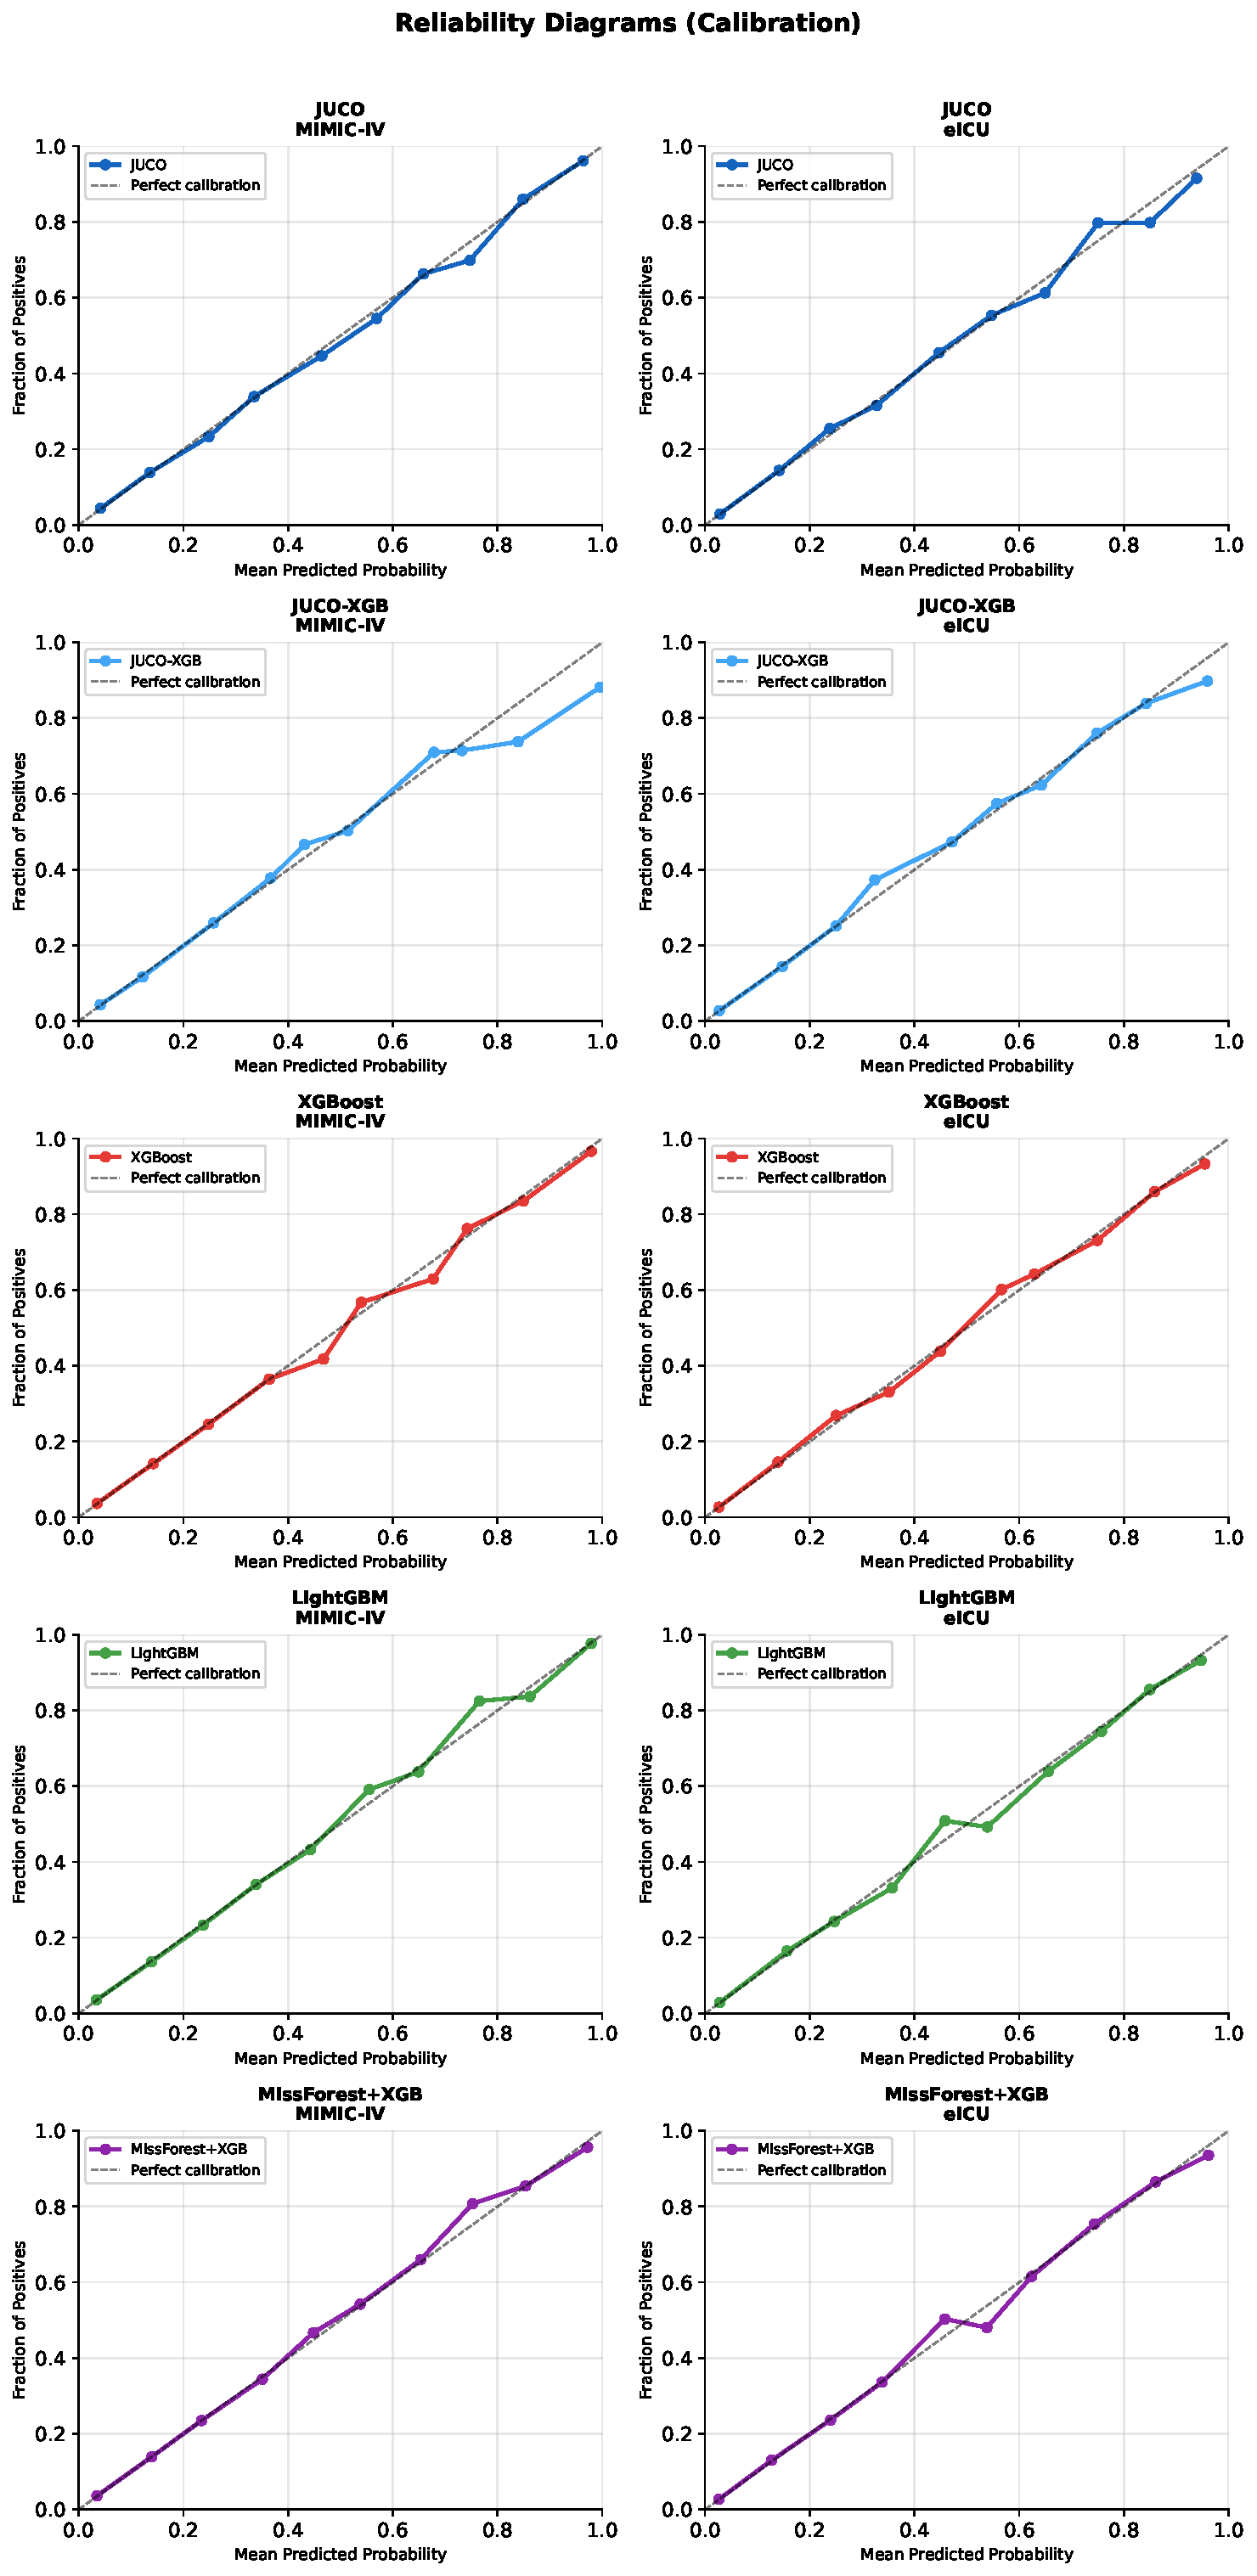
\includegraphics[width=\linewidth,
		height=0.88\textheight,keepaspectratio]{fig.pdf}
		
		\caption{Reliability diagrams for all models on
			MIMIC-IV (left column) and eICU (right column). The
			diagonal dashed line represents perfect
			calibration. JUCO achieves ECE $= 0.0063$ on
			MIMIC-IV and ECE $= 0.0029$ on eICU with frozen
			isotonic calibration parameters, demonstrating
			stable calibration under cross-institutional
			distribution shift.}
		\label{fig:reliability}
	\end{figure}
	%% =========================================================================
	%%  APPENDIX C — EXTENDED eICU COHORT STATISTICS
	%% =========================================================================
	
	\section{Extended eICU Cohort Statistics}
	\label{app:eicu_stats}

	Table~\ref{tab:eicu_stats} presents summary statistics
	for both cohorts alongside per-fold mortality rates,
	confirming that patient-level GroupKFold stratification
	produces folds with consistent mortality prevalence
	across both datasets and that the lower eICU mortality
	rate (5.32\% versus 10.58\% in MIMIC-IV) reflects
	genuine case-mix differences rather than stratification
	artefacts.
	
	
	\begin{table}[!htbp]
		\centering
		\caption{Cohort summary statistics for MIMIC-IV
			(primary) and eICU (external validation). Feature
			counts include binary missingness indicators
			appended for features with ${>}5\%$ missing rate.
			Mortality rates are computed after the 4-hour /
			30-day admission-length filter.}
		\label{tab:eicu_stats}
	\resizebox{\linewidth}{!}{%
		\begin{tabular}{lcc}
			\toprule
			\textbf{Variable} & \textbf{MIMIC-IV}
			& \textbf{eICU} \\
			\midrule
			Total ICU stays
			& 82{,}785 & 162{,}136 \\
			Unique patients
			& 63{,}687 & 121{,}567 \\
			Hospitals
			& 1 (BIDMC) & 208 \\
			In-hospital deaths
			& 8{,}762 & 8{,}621 \\
			Crude mortality, \%
			& 10.58\% & 5.32\% \\
			Raw features
			& 155 & 155 \\
			+ Missingness indicators
			& +26 & +74 \\
			Total features
			& 181 & 229 \\
			CV folds
			& 5 (patient-level) & 5 (patient-level) \\
			\midrule
			\multicolumn{3}{l}{\textit{Per-fold stays /
					deaths / mortality rate}} \\
			Fold 1
			& 16{,}557 / 1{,}792 / 10.82\%
			& 32{,}428 / 1{,}731 / 5.34\% \\
			Fold 2
			& 16{,}557 / 1{,}762 / 10.64\%
			& 32{,}427 / 1{,}729 / 5.33\% \\
			Fold 3
			& 16{,}557 / 1{,}750 / 10.57\%
			& 32{,}427 / 1{,}731 / 5.34\% \\
			Fold 4
			& 16{,}557 / 1{,}688 / 10.20\%
			& 32{,}427 / 1{,}683 / 5.19\% \\
			Fold 5
			& 16{,}557 / 1{,}770 / 10.69\%
			& 32{,}427 / 1{,}747 / 5.39\% \\
			\bottomrule
		\end{tabular}
	}
	\end{table}
	
	
	\section*{Acknowledgment}
	The authors gratefully acknowledge the use of the MIMIC-IV and eICU Collaborative Research Databases, made publicly available via PhysioNet under credentialed health data licences, without which the scale of validation reported in this paper would not have been possible. This research did not receive any specific grant from funding agencies in the public, commercial, or not-for-profit sectors.

	\bibliographystyle{IEEEtran}
	\bibliography{references}
	
\end{document}